\documentclass{beamer}

% Theme
\usetheme{ITCR}

% Encoding
\usepackage[utf8]{inputenc}

% Symbols
\usepackage{latexsym}
\usepackage{amsmath}
\usepackage{amssymb}

% Commands
\newcommand{\superscript}[1]{\ensuremath{^{\textrm{\small#1}}}}
\newcommand{\subscript}[1]{\ensuremath{_{\textrm{\small#1}}}}

% Logo
\logo{
\includegraphics[height=2cm]{style/logo.pdf}}

% Title
\begin{document}
\title{Linear programming}
\subtitle{By example}
\author{Carolina Aguilar \and Carlos Jenkins}
\date{}
\frame{\titlepage
\begin{center}
\vspace{-30mm}
{\scriptsize caroagse@gmail.com \hspace{5mm} carlos@jenkins.co.cr}\\
\vspace{10mm}
{\small Operations Research IC-6400}\\
{\small Costa Rica Institute of Technology}\\
\vspace{5mm}
{\tiny \today}
\end{center}
}

% Slides
\begin{frame}{Introduction}
FIXME: Add introduction.
\end{frame}

\begin{frame}{}
\begin{center}
{\Huge Example 01}
\end{center}
\end{frame}

\begin{frame}{Example 01 - Problem}
Farmer Jones must determine how many acres of corn and wheat to plant this year.
An acre of wheat yields 25 bushels of wheat and requires 10 hours of labor per
week. An acre of corn yields 10 bushels of corn and requires 4 hours of labor
per week. All wheat can be sold at \$4 a bushel, and all corn can be sold at
\$3 a bushel. Seven acres of land and 40 hours per week of labor are available.
Government regulations require that at least 30 bushels of corn be produced
during the current year. Formulate an LP whose solution will tell Farmer Jones
how to maximize the total revenue from wheat and corn.
\end{frame}

%\begin{frame}{Example 01 - Analisis}
\end{frame}

%\begin{frame}{Example 01 - Variables}
\Huge{
$\colora{AT} \longrightarrow$
    weat acres \\ \vspace{1cm}
$\colorb{AM} \longrightarrow$
    corn acres
}
\end{frame}

%\begin{frame}{Example 01 - Function}

Maximize the profits of planting corn and wheat :
\begin{align*}
    Z &= 100\colora{AT} + 30\colorb{AM}
\end{align*}

\end{frame}

%\begin{frame}{Example 01 - Restrictions}
\end{frame}

%\begin{frame}{Example 01 - Model}

Maximize:
\begin{align*}
    Z &= 100\colora{AT} + 30\colorb{AM}
\end{align*}

Subject to:
\begin{align*}
    10\colora{AT} + 4\colorb{AM} &\le 40 \\
      \colora{AT} +  \colorb{AM} &\le 7 \\
      \colorb{AM} &\ge 3 \\
      \colora{AT}, \colorb{AM} &\ge 0
\end{align*}

\end{frame}

%\begin{frame}{Example 01 - Solution}
\begin{figure}
    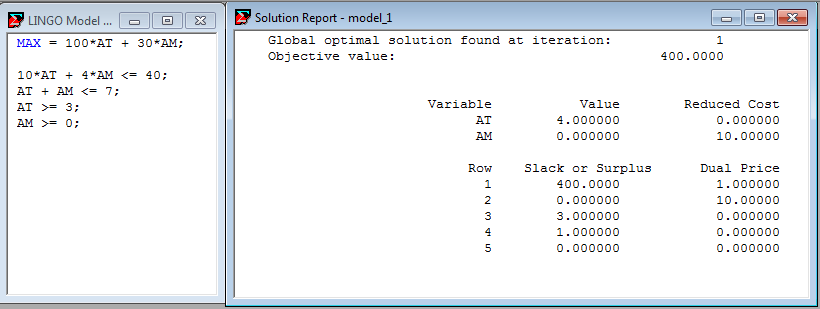
\includegraphics[width=300px]{slides/ex01/screenshot.png}
    \caption{Example 01 model and solution in Lingo Software.}
\end{figure}
\end{frame}

%\begin{frame}{Example 01 - Final solution}
\end{frame}

%\begin{frame}{Example 01 - Final analisis}

The optimal solution given by LINGO says that Farmer Jones have to plant
\textbf{4} acres of wheat and \textbf{0} acres of corn, this will generate a
profit of \textbf{\$400}. If Farmer Jones plants corn, each acre planted will
reduce the profit in \$10.

\end{frame}


%\begin{frame}{}
\begin{center}
{\Huge Example 02}
\end{center}
\end{frame}

\begin{frame}{Example 02 - Problem}
Truckco manufactures two types of trucks: 1 and 2. Each truck must go through 
the painting shop and assembly shop. If the painting shop were completely 
devoted to painting type 1 trucks, 800 per day could be painted, whereas if 
the painting shop were completely devoted to painting type 2 trucks, 700 per 
day could be painted. If the assembly shop were completely devoted to assembling 
truck 1 engines, 1500 per day could be assembled, and if the assembly shop were 
completely devoted to assembling truck 2 engines, 1200 per day could be 
assembled. Each type 1 truck contributes \$300 to profit; each type 2 truck 
contributes \$500. Formulate an LP that will maximize Truckco's profit.
\end{frame}

\begin{frame}{Example 02 - Analisis}

We must maximize the profit of the company;. TruckCo manufactures
two typesof trucks: type 1 and type 2. Each truck type 1 can be sold
at \$300 and each truck type 2 at \$500 .


\end{frame}

\begin{frame}{Example 02 - Variables}
\Huge{
$\colora{{x}_{1}} \longrightarrow$
    type 1 trucks \\ \vspace{1cm}
$\colorb{{x}_{2}} \longrightarrow$
    type 2 trucks
}
\end{frame}

\begin{frame}{Example 02 - Function}

Maximize TruckCo's profits:
\begin{align*}
    Z &= 300\colora{x_1} + 500\colorb{x_2}
\end{align*}

\end{frame}

\begin{frame}{Example 02 - Restrictions}
\end{frame}

\begin{frame}{Example 02 - Model}

\begin{itemize}
\item{Maximize: \\}
\item{$Z=300x_1+ 500x_2$ \\}
\item{Subject to: \\}
\item{$\frac { 1 }{ 800 } x_{ 1 } + \frac { 1 }{ 700 } x_{ 2 } \le 1$\\}
\item{$ \frac { 1 }{ 1500 } x_{ 1 }\quad +\quad \frac { 1 }{ 1200 } x_{ 2 }\le 1$\\}
\item{$x_{ 1 },x_{ 2 }\quad \ge \quad 0$\\}
\end{itemize}

\end{frame}


\begin{frame}{Example 02 - Solution}
\begin{figure}
    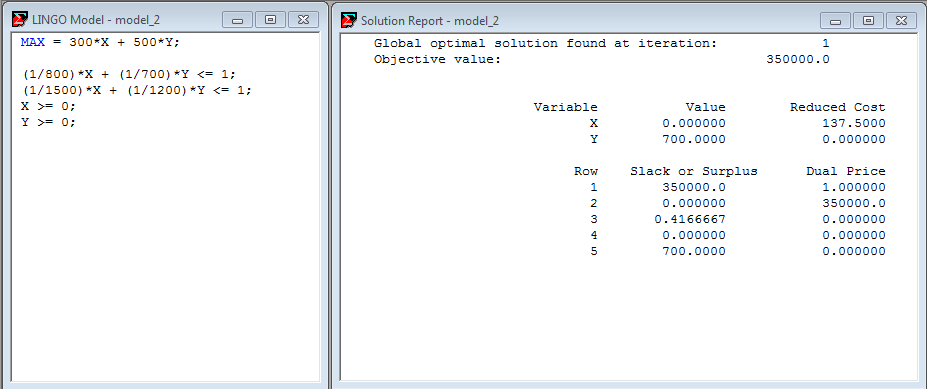
\includegraphics[width=300px]{slides/ex02/screenshot.png}
    \caption{Example 02 model and solution in Lingo Software.}
\end{figure}
\end{frame}

\begin{frame}{Example 02 - Final solution}
\end{frame}

\begin{frame}{Example 02 - Final analisis}
\end{frame}



%\begin{frame}{}
\begin{center}
{\Huge Example 03}
\end{center}
\end{frame}

\begin{frame}{Example 03 - Problem}
Leary Chemical manufactures three chemicals: A, B and C. These chemicals are 
produced via two production processes: 1 and 2. Running process 1 for an hour 
costs \$4 and yields 3 units of A, 1 of B, and 1 of C. Running process 2 for 
an hour costs \$1 and produces 1 unit of A and 1 of B. To meet customer demands, 
at least 10 units of A, 5 of B, and 3 of C must be produced daily. Graphically 
determine a daily production plan that minimizes the cost meeting Leary 
Chemical's daily demands.
\end{frame}

\begin{frame}{Example 03 - Analisis}
\end{frame}

\begin{frame}{Example 03 - Variables}
\end{frame}

\begin{frame}{Example 03 - Function}
\end{frame}

\begin{frame}{Example 03 - Restrictions}
\end{frame}

\begin{frame}{Example 03 - Model}

Minimize:
\begin{align*}
    Z &= 4\colora{x_1} + \colorb{x_2}
\end{align*}

Subject to:
\begin{align*}
    3\colora{x_1} + \colorb{x_2} &\ge 10 \\
     \colora{x_1} + \colorb{x_2} &\ge 5 \\
     \colora{x_1} &\ge 3 \\
     \colora{x_1}, \colorb{x_2} &\ge 0
\end{align*}

\end{frame}

\begin{frame}{Example 03 - Solution}
\begin{figure}
    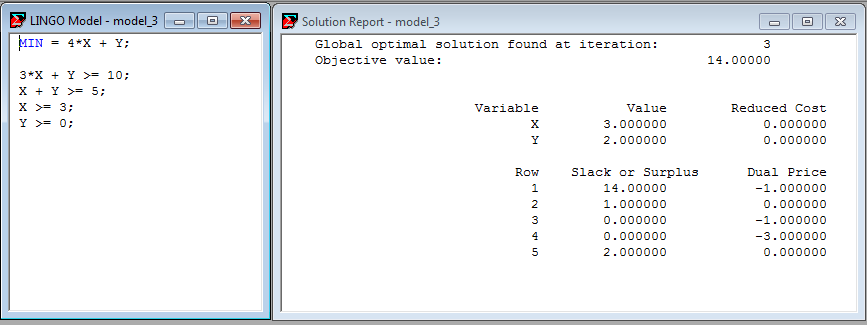
\includegraphics[width=300px]{slides/ex03/screenshot.png}
    \caption{Example 03 model and solution in Lingo Software.}
\end{figure}
\end{frame}

\begin{frame}{Example 03 - Final solution}

\colorb{Global optimal solution found at iteration:}  3\\
\colorb{Objective value:}  14.00000\\

\begin{columns}[t]
\begin{column}{0.3\textwidth}
\colorb{Variable}\\
X\\
Y\\
-----------\\
\colorb{Row}\\
1\\
2\\
3\\
4\\
5\\

\end{column}
\begin{column}{0.3\textwidth}
\colorb{Value}\\
3.000000\\
2.000000\\
-----------\\

\colorb{Slack or Surplus}\\
14.00000\\
1.000000\\
0.000000\\
0.000000\\
2.000000\\

\end{column}

\begin{column}{0.3\textwidth}
\colorb{Reduced Cost}\\
0.000000\\
0000000\\

-----------\\
\colorb{Dual Price}\\
-1.000000\\
0.000000\\
-1.000000\\
-3.000000\\
0.000000\\
\end{column}
\end{columns}
\end{frame}

\begin{frame}{Example 03 - Final analisis}
The optimal solution given by LINGO says that the two production processes of Leary Chemicals
might use 3 hours (Process 1) and 2 hours (Process 2). It will generate a cost of \$14  on daily demands.
\end{frame}



%\begin{frame}{}
\begin{center}
{\Huge Example 04}
\end{center}
\end{frame}

\begin{frame}{Example 04 - Problem}
Farmer Jane owns 45 acres of land. She is going to plant each with wheat or 
corn. Each acre planted with wheat yields \$200 profit; each with corn yields 
\$300 profit. The labor and fertilizer used for each acre are given in the 
following table. One hundred workers and 120 tons of fertilizer are available. 
Use LP to determine how Jane can maximize profits from her land.

\begin{center}
\begin{tabular}{lll}
\hline
  \cellcolor{gray90}\textbf{Resource} 
& \cellcolor{gray90}\textbf{Wheat} 
& \cellcolor{gray90}\textbf{Corn} \\
\hline
Labor      & 3 workers & 2 workers \\
Fertilizer & 2 tons    & 4 tons \\
\hline 
\end{tabular}
\end{center}

\end{frame}

\begin{frame}{Example 04 - Analisis}

We must maximize profits from Jane land. We know each acre of wheat yields \$200
and each acre of corn yields \$300.
So we need to maximize 200*EachAcreOfWheat + 300*EachAcreOfCorn.

\end{frame}

\begin{frame}{Example 04 - Variables}
\Huge{
$\textcolor{deepred}  {{x}_{1}} \longrightarrow$
    weat acres \\ \vspace{1cm}
$\textcolor{deepgreen}{{x}_{2}} \longrightarrow$
    corn acres
}
\end{frame}

\begin{frame}{Example 04 - Function}
\end{frame}

\begin{frame}{Example 04 - Restrictions}

The first restriction is about the acres available in Jane's Farm. She owns
45 acres of land, so $\colora{AT} +  \colorb{AM} \le 45$. Also there is
restricted the amount of workers available, there are 100 workers and for
wheat production there are needed 3 workers and for corn production
there are needed 2 workers; so these could be expressed as $3\colora{AT} + 2\colorb{AM} \le 100$.
Also wheat needs 2 tons of fertilizer, corn needs 4 tons, and there are just
120 tons of fertilizer available , so $2\colora{AT} + 4\colorb{AM} \le 120$.
Then we have the last restriction that all variables must be greater or equal
than 0.
\end{frame}

\begin{frame}{Example 04 - Model}
\end{frame}

\begin{frame}{Example 04 - Solution}
\begin{figure}
    \includegraphics[width=300px]{slides/ex04/screenshot.png}
    \caption{Example 04 model and solution in Lingo Software.}
\end{figure}
\end{frame}

\begin{frame}{Example 04 - Final solution}

\colorb{Global optimal solution found at iteration:}  2\\
\colorb{Objective value:}  10000.00\\

\begin{columns}[t]
\begin{column}{0.3\textwidth}
\colorb{Variable}\\
AT\\
AM\\
-----------\\
\colorb{Row}\\
1\\
2\\
3\\
4\\
5\\
6\\

\end{column}
\begin{column}{0.3\textwidth}
\colorb{Value}\\
20.00000\\
20.00000\\

-----------\\
\colorb{Slack or Surplus}\\
10000.00\\
5.000000\\
0.000000\\
0.000000\\
20.00000\\
20.00000\\

\end{column}

\begin{column}{0.3\textwidth}
\colorb{Reduced Cost}\\
0.000000\\
0.000000\\

-----------\\
\colorb{Dual Price}\\
1.000000\\
0.000000\\
25.00000\\
62.50000\\
0.000000\\
0.000000\\
\end{column}
\end{columns}
\end{frame}

\begin{frame}{Example 04 - Final analisis}
The optimal solution given by LINGO says that FarmerJane must plant  20 acres of wheat  and
20 acres of corn to maximize profits from her land. It will generate a profit of \$10000.
\end{frame}



%\begin{frame}{}
\begin{center}
{\Huge Example 05}
\end{center}
\end{frame}

\begin{frame}{Example 05 - Problem (1)}
There are three factories on the Momiss River (1, 2 and 3). Each emits two types
of pollutants (1 and 2) into the river. If the waste from each factory is 
processed, the pollution in the river can be reduced. It costs \$15 to process a
ton of factory 1 waste, and each ton processed reduces the amount of pollutant 1
by 0.10 ton and the amount of pollutant 2 by 0.45 ton. It costs \$10 to process
a ton of factory 2 waste, and each ton processed will reduce the amount of 
pollutant 1 by 0.20 ton and the amount of pollutant 2 by 0.25 ton. It costs \$20
to process a ton of factory 3 waste, and each ton processed will reduce the 
amount of pollutant 1 by 0.40 ton and the amount of pollutant 2 by 0.30 ton.
\end{frame}

\begin{frame}{Example 05 - Problem (2)}
The state wants to reduce the amount of pollutant 1 in the river by at least 30 
tons and the amount of pollutant 2 in the river by at least 40 tons. Formulate 
an LP that will minimize the cost of reducing pollution by the desired amounts.

\begin{center}
\begin{tabular}{|c||c|c|c|}
\hline
& \cellcolor{gray90}\textbf{Factory 1} 
& \cellcolor{gray90}\textbf{Factory 2} 
& \cellcolor{gray90}\textbf{Factory 3} \\
\hline
\hline \cellcolor{gray90}\textbf{Cost per ton}  & 15   & 10   & 20   \\
\hline \cellcolor{gray90}\textbf{Contaminant 1} & 0.10 & 0.20 & 0.40 \\
\hline \cellcolor{gray90}\textbf{Contaminant 2} & 0.45 & 0.25 & 0.30 \\
\hline 
\end{tabular}
\end{center}

\end{frame}

\begin{frame}{Example 05 - Analisis}
\end{frame}

\begin{frame}{Example 05 - Variables}
\end{frame}

\begin{frame}{Example 05 - Function}
\end{frame}

\begin{frame}{Example 05 - Restrictions}
\end{frame}

\begin{frame}{Example 05 - Model}

Minimize:
\begin{align*}
    Z &= 15\colora{x} + 10\colorb{y} + 20\colorc{z}
\end{align*}

Subject to:
\begin{align*}
    0.1 \colora{x} + 0.2 \colorb{y} + 0.4\colorc{z} &\ge 30 \\
    0.45\colora{x} + 0.25\colorb{y} + 0.3\colorc{z} &\ge 40 \\
        \colora{x}, \colorb{y}, \colorc{z} &\ge 0
\end{align*}

\end{frame}

\begin{frame}{Example 05 - Solution}
\begin{figure}
    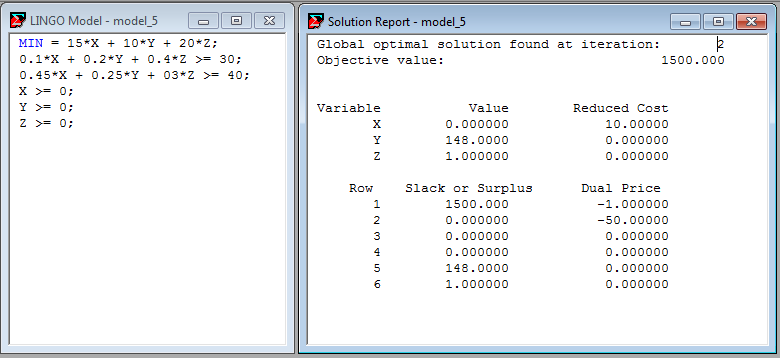
\includegraphics[width=300px]{slides/ex05/screenshot.png}
    \caption{Example 05 model and solution in Lingo Software.}
\end{figure}
\end{frame}

\begin{frame}{Example 05 - Final solution}

\colorb{Global optimal solution found at iteration:}  2\\
\colorb{Objective value:}  1500.000\\

\begin{columns}[t]
\begin{column}{0.3\textwidth}
\colorb{Variable}\\
X\\
Y\\
Z\\
-----------\\
\colorb{Row}\\
1\\
2\\
3\\
4\\
5\\
6\\

\end{column}
\begin{column}{0.3\textwidth}
\colorb{Value}\\
0.000000 \\
148.0000\\
1.000000\\

-----------\\
\colorb{Slack or Surplus}\\
1500.000\\
0.000000\\
0.000000\\
0.000000\\
148.0000\\
1.000000\\

\end{column}  

\begin{column}{0.3\textwidth}
\colorb{Reduced Cost}\\
10.00000\\
0.000000\\
0.000000\\

-----------\\
\colorb{Dual Price}\\
-1.000000\\
-50.00000\\
0.000000\\
0.000000\\
0.000000\\
0.000000\\
\end{column}
\end{columns}  
\end{frame}

\begin{frame}{Example 05 - Final analisis}
\end{frame}



%\begin{frame}{}
\begin{center}
{\Huge Example 06}
\end{center}
\end{frame}

\begin{frame}{Example 06 - Problem}
\end{frame}

\begin{frame}{Example 06 - Analisis}
U.S Labs purchases the valves from 3 different suppliers. Each of
these suppliers sells the valves at different prices. Supplier 1 sells the
valves at a cost per value of \$5, Supplier 2 sells them at \$4 and the last
one, Supplier 3 sells the valves at \$3. U.S labs needs to minimize the cost
of acquiring the needed valves, so it could be expressed as minimize
\$5*ValvesFromSupplier1 + \$4*ValvesFromSupplier2 +
\$3*ValvesFromSupplier3

\end{frame}

\begin{frame}{Example 06 - Variables}
\end{frame}

\begin{frame}{Example 06 - Function}
\end{frame}

\begin{frame}{Example 06 - Restrictions}
\end{frame}

\begin{frame}{Example 06 - Model}
\end{frame}

\begin{frame}{Example 06 - Solution}
\end{frame}

\begin{frame}{Example 06 - Final solution}
\footnotesize
\colorb{Global optimal solution found at iteration:} \\
\colorb{Objective value:}  \\

\begin{columns}[t]
\begin{column}{0.3\textwidth}
\colorb{Variable}\\
V1\\
V2\\
V3\\
-----------\\
\colorb{Row}\\
1\\
2\\
3\\
4\\
5\\
6\\
7\\
8\\
9\\
10\\

\end{column}
\begin{column}{0.3\textwidth}
\colorb{Value}\\
500.000\\
500.000\\
500.000\\
-----------\\
\colorb{Slack or Surplus}\\
0.00000\\
-50.0000\\
175.000\\
275.000\\
0.00000\\
0.00000\\
0.00000\\
500.000\\
500.000\\
500.000\\
\end{column}  

\begin{column}{0.3\textwidth}
\colorb{Reduced Cost}\\
0.00000\\
0.00000\\
0.00000\\

-----------\\
\colorb{Dual Price}\\
-1.000000\\
-0.2000000E+11\\
0.000000\\
0.000000\\
0.8000000E+10\\
0.6000000E+10\\
0.4000000E+10\\
0.000000\\
0.000000\\
0.000000\\                              
\end{column}
\end{columns}  


\end{frame}

\begin{frame}{Example 06 - Final analisis}
LINGO detects an "Unbounded Solution" in the model.
When the “Unbounded Solution” termination occurs, it implies the formulation
admits the unrealistic result  that an infinite amount of profit can be made. A more
realistic conclusion is that an important  constraint has been omitted or the
formulation contains a critical typographical error.
\end{frame}



%\begin{frame}{}
\begin{center}
{\Huge Example 07}
\end{center}
\end{frame}

\begin{frame}{Example 07 - Problem}
Highland's TV-Radio Store must determine how many TVs and radios to keep in 
stock. A TV requires 10 sq ft of floorspace, whereas a radio requires 4 sq ft; 
200 sq ft of floorspace is available. A TV will earn Highland \$60 in profits, 
and a radio will earn \$20. The store stocks only TVs and radios. Marketing 
requirements dictate that at least 60\% of all appliances in stock be radios. 
Finally, a TV ties up \$200 in capital, and a radio, \$50. Highland wants to 
have at most \$3000 worth of capital tied up at any time. Formulate an LP that 
can be used to maximize Highland's profit.

\begin{center}
\begin{tabular}{|c||c|c|c|}
\hline
& \cellcolor{gray90}\textbf{Required space} 
& \cellcolor{gray90}\textbf{Profit} 
& \cellcolor{gray90}\textbf{Capital} \\
\hline
\hline \cellcolor{gray90}\textbf{TV}    & 10 & \$60 & \$200 \\
\hline \cellcolor{gray90}\textbf{Radio} &  4 & \$20 &  \$50 \\
\hline 
\end{tabular}
\end{center}

\end{frame}

\begin{frame}{Example 07 - Analisis (1)}

The previous problem statement can be represented with the following table:

\begin{center}
\begin{tabular}{lrrr}
\hline
  \cellcolor{gray90}\textbf{Item}
& \cellcolor{gray90}\textbf{Required space}
& \cellcolor{gray90}\textbf{Profit}
& \cellcolor{gray90}\textbf{Capital} \\
\hline
TV    & 10 & \$60 & \$200 \\
Radio &  4 & \$20 &  \$50 \\
\hline
\end{tabular}
\end{center}

\end{frame}

\begin{frame}{Example 07 - Analisis (2)}
We need to maximize Highland's TV-Radio Store profits. We know that
each TV sold yields \$60 and each radio sold yields \$20. So the profit
to maximize could be represented as \$60*TVsInStock + \$20RadiosInStock

\end{frame}

\begin{frame}{Example 07 - Variables}
\end{frame}

\begin{frame}{Example 07 - Function}

Maximize Highland's TV-Radio Store profit:
\Huge{
\begin{align*}
    Z &= 60\colora{TV} + 20\colorb{R}
\end{align*}
}

\end{frame}

\begin{frame}{Example 07 - Restrictions}

The first restriction would be about the space available in the store and the
space both TVs and radios requires. There is 200ft\superscript{2} available and
a TV requires 10ft\superscript{2} and a radio requires 4ft\superscript{2}; from
there we have the restriction $10\colora{TV} + 4\colorb{R} \le 200$. Another
restriction is about the requires that from marketing, which would give the
equation: $\frac{\colorb{R}}{\colora{TV} + \colorb{R}} \ge 0.6$. Futhermore,
the are presented by the fact that Highlands want to invest un maximum of \$3000
in capital and both TVs and radios requires \$200 and \$50 respectively; that
gives the restriction: $200\colora{TV} + 50\colorb{R} \le 3000$. Finally we
need not to forget the trivial restriction that both TVs and radios needs to be
positive as we can buy negative things.

\end{frame}

\begin{frame}{Example 07 - Model}
\end{frame}

\begin{frame}{Example 07 - Solution}
\begin{figure}
    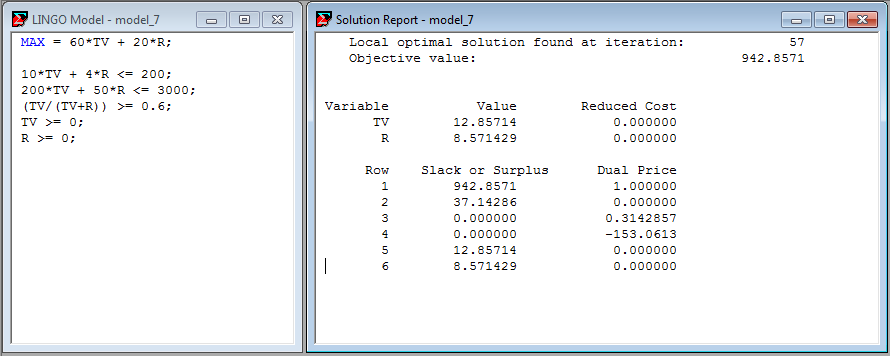
\includegraphics[width=300px]{slides/ex07/screenshot.png}
    \caption{Example 07 model and solution in Lingo Software.}
\end{figure}
\end{frame}

\begin{frame}{Example 07 - Final solution}

\footnotesize
\colorb{Global optimal solution found at iteration:} 57\\
\colorb{Objective value:}  942.8571\\

\begin{columns}[t]
\begin{column}{0.3\textwidth}
\colorb{Variable}\\
TV\\
R\\
-----------\\
\colorb{Row}\\
1\\
2\\
3\\
4\\
5\\
6\\

\end{column}
\begin{column}{0.3\textwidth}
\colorb{Value}\\
12.85714\\
8.571429\\

-----------\\
\colorb{Slack or Surplus}\\
942.8571\\
37.14286\\
0.000000\\
0.000000\\
12.85714\\
8,571429\\

\end{column}

\begin{column}{0.3\textwidth}
\colorb{Reduced Cost}\\
0.000000\\
0.000000\\

-----------\\
\colorb{Dual Price}\\
1.000000\\
0.000000\\
0.3142857\\
-153.0613\\
0.000000\\
0.000000\\
\end{column}
\end{columns}
\end{frame}

\begin{frame}{Example 07 - Final analisis}
\end{frame}



%\begin{frame}{}
\begin{center}
{\Huge Example 08}
\end{center}
\end{frame}

\begin{frame}{Example 08 - Problem}
\end{frame}

\begin{frame}{Example 08 - Analisis}
\end{frame}

\begin{frame}{Example 08 - Variables}
\begin{center}
\Huge{
$\textcolor{deepred}{X}_{\textcolor{deepgreen}{i}, \textcolor{deepblue}{j}}$
}
\end{center}
\large{
$\textcolor{deepred}  {X} \longrightarrow$
    tons of coal  \\ \vspace{1cm}
$\textcolor{deepgreen}{i} \longrightarrow$
    mine number from where the coal will be extrated [1;3] \\ \vspace{1cm}
$\textcolor{deepblue} {j} \longrightarrow$
    number of customer [1;4]
}
\end{frame}

\begin{frame}{Example 08 - Function}

Minimize the cost of meeting customer coal demands:
\Large{
\begin{align*}
    Z =& 200\colorij{X}{1}{1} + 300\colorij{X}{1}{2} + 400\colorij{X}{1}{3} + 600\colorij{X}{1}{4} + \\
       & 495\colorij{X}{2}{1} + 330\colorij{X}{2}{2} + 385\colorij{X}{2}{3} + 605\colorij{X}{2}{4} + \\
       & 496\colorij{X}{3}{1} + 744\colorij{X}{3}{2} + 186\colorij{X}{3}{3} + 310\colorij{X}{3}{4}
\end{align*}
}

\end{frame}

\begin{frame}{Example 08 - Restrictions}

The first restrictions are quite straightforward, the first 4 restrictions are
(see model in the next slide) restrict the demand from clients (1, 2, 3 and 4).
The following 3 equations restrict the capacity of the mine (1, 2 and 3). The
final two restrictions are the more complicated ones, the first one restricts
the percentage of ash in the coal, and the next one restrict the percentage of
sulfur in the coal.

\end{frame}

\begin{frame}{Example 08 - Model (1)}

Minimize:
\begin{align*}
    Z =& 200\colorij{X}{1}{1} + 300\colorij{X}{1}{2} + 400\colorij{X}{1}{3} + 600\colorij{X}{1}{4} + \\
       & 495\colorij{X}{2}{1} + 330\colorij{X}{2}{2} + 385\colorij{X}{2}{3} + 605\colorij{X}{2}{4} + \\
       & 496\colorij{X}{3}{1} + 744\colorij{X}{3}{2} + 186\colorij{X}{3}{3} + 310\colorij{X}{3}{4}
\end{align*}

Subject to:
\small{
\begin{align*}
    \colorij{X}{1}{1} + \colorij{X}{2}{1} + \colorij{X}{3}{1} &= 80 \\
    \colorij{X}{1}{2} + \colorij{X}{2}{2} + \colorij{X}{3}{2} &= 70 \\
    \colorij{X}{1}{3} + \colorij{X}{2}{3} + \colorij{X}{3}{3} &= 60 \\
    \colorij{X}{1}{4} + \colorij{X}{2}{4} + \colorij{X}{3}{4} &= 90 \\
    %
    \colorij{X}{1}{1} + \colorij{X}{1}{2} + \colorij{X}{1}{3} + \colorij{X}{1}{4} &\le 120 \\
    \colorij{X}{2}{1} + \colorij{X}{2}{2} + \colorij{X}{2}{3} + \colorij{X}{2}{4} &\le 100 \\
    \colorij{X}{3}{1} + \colorij{X}{3}{2} + \colorij{X}{3}{3} + \colorij{X}{3}{4} &\le 140 \\
    %
    \colorij{X}{i}{j} &\ge 0
\end{align*}
}

\end{frame}

\begin{frame}{Example 08 - Model (2)}

And...

\tiny{
\begin{align*}
    \frac{
        0.8(\colorij{X}{1}{1} + \colorij{X}{1}{2} + \colorij{X}{1}{3} + \colorij{X}{1}{4}) +
        0.6(\colorij{X}{2}{1} + \colorij{X}{2}{2} + \colorij{X}{2}{3} + \colorij{X}{2}{4}) +
        0.4(\colorij{X}{3}{1} + \colorij{X}{3}{2} + \colorij{X}{3}{3} + \colorij{X}{3}{4})
    }{
        \colorij{X}{1}{1} + \colorij{X}{1}{2} + \colorij{X}{1}{3} + \colorij{X}{1}{4} +
        \colorij{X}{2}{1} + \colorij{X}{2}{2} + \colorij{X}{2}{3} + \colorij{X}{2}{4} +
        \colorij{X}{3}{1} + \colorij{X}{3}{2} + \colorij{X}{3}{3} + \colorij{X}{3}{4}
    } &\le 0.05
\end{align*}

\begin{align*}
    %
    \frac{
        0.5(\colorij{X}{1}{1} + \colorij{X}{1}{2} + \colorij{X}{1}{3} + \colorij{X}{1}{4}) +
        0.4(\colorij{X}{2}{1} + \colorij{X}{2}{2} + \colorij{X}{2}{3} + \colorij{X}{2}{4}) +
        0.3(\colorij{X}{3}{1} + \colorij{X}{3}{2} + \colorij{X}{3}{3} + \colorij{X}{3}{4})
    }{
        \colorij{X}{1}{1} + \colorij{X}{1}{2} + \colorij{X}{1}{3} + \colorij{X}{1}{4} +
        \colorij{X}{2}{1} + \colorij{X}{2}{2} + \colorij{X}{2}{3} + \colorij{X}{2}{4} +
        \colorij{X}{3}{1} + \colorij{X}{3}{2} + \colorij{X}{3}{3} + \colorij{X}{3}{4}
    } &\le 0.04
\end{align*}
}
\end{frame}

\begin{frame}{Example 08 - Solution}
%\begin{figure}
    %\includegraphics[width=300px]{slides/ex08/screenshot.png}
    %\caption{Example 08 model and solution in Lingo Software.}
%\end{figure}
\end{frame}

\begin{frame}{Example 08 - Final solution}

\colorb{Global optimal solution found at iteration:} \\
\colorb{Objective value:}  \\

\begin{columns}[t]
\begin{column}{0.3\textwidth}
\colorb{Variable}\\
X11\\
X12\\
X13\\
X14\\
X21\\
X22\\
X23\\
X24\\
X31\\
X32\\
X33\\
X34\\
-----------\\
\colorb{Row}\\
1\\
2\\
3\\
4\\
5\\
6\\
7\\
8\\
9\\
10\\
11\\
12\\
13\\
14\\
15\\
16\\
17\\
18\\
19\\
20\\
21\\
22\\

\end{column}
\begin{column}{0.3\textwidth}
\colorb{Value}\\
60.00000\\
0.000000\\
0.000000\\
0.000000\\
9.999999\\
70.00000\\
20.00000\\
0.000000\\
10.00000\\
0.000000\\
40.00000\\
90.00000\\
-----------\\
\colorb{Slack or Surplus}\\
18810.00\\
-0.3722023E-07\\
-0.2381191E-07\\
-0.3231968E-07\\
-0.1268634E-06\\
60.00000\\
0.000000\\
0.000000\\
-0.4966667\\
-0.3333333\\
60.00000\\
0.000000\\
0.000000\\
0.000000\\
9.999999\\
70.00000\\
20.00000\\
0.000000\\
10.00000\\
0.000000\\
40.00000\\
90.00000\\

\end{column}  

\begin{column}{0.3\textwidth}
\colorb{Reduced Cost}\\
0.000000\\
0.000000\\
0.000000\\
0.000000\\
0.000000\\
0.000000\\
0.000000\\
0.000000\\
0.000000\\
0.000000\\
0.000000\\
0.000000\\


-----------\\
\colorb{Dual Price}\\
-1.000000\\
-0.1266667E-02\\
-0.1266667E-02\\
-0.1266667E-02\\
-0.1266667E-02\\
0.000000\\
0.9999999E-03\\
0.2000000E-02\\
1.000000\\
1.000000\\
0.000000\\
0.000000\\
0.000000\\
0.000000\\
0.000000\\
0.000000\\
0.000000\\
0.000000\\
0.000000\\
0.000000\\
0.000000\\
0.000000\\

                           
\end{column}
\end{columns}  

\end{frame}

\begin{frame}{Example 08 - Final analisis}
\end{frame}



%\begin{frame}{}
\begin{center}
{\Huge Example 09}
\end{center}
\end{frame}

\begin{frame}{Example 09 - Problem}
\end{frame}

\begin{frame}{Example 09 - Analisis}

The solution asked is about maximize the contribution to profit from manufacturing
tables and chairs. Each unfinished table can be sold at \$70 (70*UT), each finished
table at \$140 (140*FT), an unfinished chair can be sold at \$60 (60*UC) and a finished
chair at \$110 (110*FC). But we need to deduct from these profits the cost of buying
the wood require to manufacture the chairs and tables. Each board ft of wood may be
purchased at \$1, so a table requires 40 board ft that means \$40*(FT + UT); a chair requires
30 board ft of wood so: \$30*(FC + UC). Now putting all together we have that the function
to maximize is MAX Z= 70UT + 140FT + 60UC + 110FC-40(FT+UT)-30(FC+UC).

\end{frame}

\begin{frame}{Example 09 - Variables}
\large{
$\colora{UT} \longrightarrow$
    unfinished table  \\ \vspace{1cm}
$\colorb{FT} \longrightarrow$
    finished table \\ \vspace{1cm}
$\colorc{UC} \longrightarrow$
    unfinished chair \\ \vspace{1cm}
$\colord{FC} \longrightarrow$
    finished char
}
\end{frame}

\begin{frame}{Example 09 - Function}

Maximize the contribution to Furnco profit from manufacturing tables and chairs:
\begin{align*}
    Z = &70\colora{UT} + 140\colorb{FT} + 60\colorc{UC} + 110\colord{FC} - \\
        &40(\colorb{FT} + \colora{UT}) - 30(\colord{FC} + \colorc{UC})
\end{align*}

\end{frame}

\begin{frame}{Example 09 - Restrictions}
\end{frame}

\begin{frame}{Example 09 - Model}

Maximize:
\begin{align*}
    Z = &70\colora{UT} + 140\colorb{FT} + 60\colorc{UC} + 110\colord{FC} - \\
        &40(\colorb{FT} + \colora{UT}) - 30(\colord{FC} + \colorc{UC})
\end{align*}

Subject to:
\begin{align*}
    40(\colorb{FT} + \colora{UT}) + 30(\colord{FC} + \colorc{UC}) &\le 40000 \\
    5\colorb{FT} + 2\colora{UT} + 4\colord{FC} + 2\colorc{UC} &\le 6000
\end{align*}

\end{frame}

\begin{frame}{Example 09 - Solution}
\end{frame}

\begin{frame}{Example 09 - Final solution}
\footnotesize
\colorb{Global optimal solution found at iteration:} 2 \\
\colorb{Objective value:}  106666.7\\

\begin{columns}[t]
\begin{column}{0.3\textwidth}
\colorb{Variable}\\
UT\\
FT\\
UC\\
FC\\
-----------\\
\colorb{Row}\\
1\\
2\\
3\\
4\\
5\\
6\\
7\\

\end{column}
\begin{column}{0.3\textwidth}
\colorb{Value}\\
0.000000\\
0.000000\\
0.000000\\
1333.333\\

-----------\\
\colorb{Slack or Surplus}\\
106666.7\\
0.000000\\
666.6667\\
0.000000\\
0.000000\\
1333.333\\
0.000000\\

\end{column}

\begin{column}{0.3\textwidth}
\colorb{Reduced Cost}\\
76.66667\\
6.666667\\
50.00000\\
0.000000\\


-----------\\
\colorb{Dual Price}\\
1.000000\\
2.666667\\
0.000000\\
0.000000\\
0.000000\\
0.000000\\
0.000000\\

\end{column}
\end{columns}
\end{frame}

\begin{frame}{Example 09 - Final analisis}
The optimal solution given by LINGO says that Furnco must manufacture
0 unfinished tables, 0 finished tables, 0 unfinished chairs and  1333.333 finished chairs.
It will generate the optimal profit of \$106666.7. Each unfinished table manufactured
will reduce the profit by \$76.66667, each finished table by \$6.66667 and each
unfinished table by \$50.
\end{frame}



%\begin{frame}{}
\begin{center}
{\Huge Example 10}
\end{center}
\end{frame}

\begin{frame}{Example 10 - Problem (1)}
A company produces six products in the following fashion. Each unit of raw
material purchased yields four units of product 1, two units of product 2, and
one unit of product 3. Up to 1200 units of product 1 can be sold, and up to 300
units of product 2 can be sold. Each unit of product 1 can be sold or processed
further. Each unit of product 1 that is processed yields a unit of product 4.
Demand for products 3 and 4 is unlimited. Each unit of product 2 can be sold or
processed further. Each unit of product 2 that is processed further yields 0.8
unit of product 5 and 0.3 unit of product 6. Up to 1000 units of product 5 can
be sold, and up to 800 units of product 6 can be sold. Up to 3000 units of raw
material can be purchased at \$6 per unit.
\end{frame}

\begin{frame}{Example 10 - Problem (2)}
Leftover units of products 5 and 6 must be destroyed. It costs \$4 to destroy
each leftover unit of product 5 and \$3 to destroy each leftover unit of product
6. Ignoring raw material purchase costs, the per-unit sales price and production
costs for each product are shown in the following table. Formulate an LP whose
solution will yield a profit-maximizing production schedule.

\begin{center}
\begin{tabular}{lrrr}
\hline
  \cellcolor{gray90}\textbf{Product}
& \cellcolor{gray90}\textbf{Sales price}
& \cellcolor{gray90}\textbf{Production cost} \\
\hline
Product 1 &  \$7 & \$4 \\
Product 2 &  \$6 & \$4 \\
Product 3 &  \$4 & \$2 \\
Product 4 &  \$3 & \$1 \\
Product 5 & \$20 & \$5 \\
Product 6 & \$35 & \$5 \\
\hline
\end{tabular}
\end{center}

\end{frame}

\begin{frame}{Example 10 - Analisis}
\end{frame}

\begin{frame}{Example 10 - Variables}
\begin{multicols}{3}

\begin{center}
\Huge{
$\textcolor{deepred}{x}_{\textcolor{deepgreen}{i}}$
}
\end{center}
\normalsize{
$\textcolor{deepred}  {x} \longrightarrow$
    amount of product to produce  \\
$\textcolor{deepgreen}{i} \longrightarrow$
    number of product to produce [1;6]
}
\vfill
\columnbreak


\begin{center}
\Huge{
$\textcolor{deepred}{d}_{\textcolor{deepgreen}{i}}$
}
\end{center}
\normalsize{
$\textcolor{deepred}  {d} \longrightarrow$
    amount of product to destroy  \\
$\textcolor{deepgreen}{i} \longrightarrow$
    number of product to destroy [1;6]
}
\vfill
\columnbreak


\begin{center}
\Huge{
$\textcolor{deepred}{m}$
}
\end{center}
\normalsize{
$\textcolor{deepred}  {m} \longrightarrow$
    amount of material to buy
}

\end{multicols}
\end{frame}

\begin{frame}{Example 10 - Function}

Get a profit-maximizing production schedule:
\Huge{
\begin{align*}
    Z =& 3\colora{x_1} + 2 \colora{x_2} + 2 \colora{x_3} + \\
       & 2\colora{x_4} + 15\colora{x_5} + 30\colora{x_6} - \\
       & 4\colorb{d_1} - 3 \colorb{d_2} - 6 \colorc{m}
\end{align*}
}

\end{frame}

\begin{frame}{Example 10 - Restrictions}

This problem has many restrictions, so we will enumerate them accordingly to
their position in the next slide (model):

\begin{enumerate}
\item Restricts the amount of material that can be bought.
\item Restricts the amount of products that M can generate.
\item Another equation that restricts the amount of products that M can generate.
\item And yet another one.
\item Restricts the amount of type 1 products to create.
\item Restricts the amount of type 2 products to create.
\item Restricts the amount of type 5 products to create.
\item Restricts the amount of type 6 products to create.
\item The final and trivial restrictions.
\end{enumerate}

\end{frame}

\begin{frame}{Example 10 - Model}

Maximize:
\begin{align*}
    Z &= 3\colora{x_1} + 2 \colora{x_2} + 2 \colora{x_3} +
         2\colora{x_4} + 15\colora{x_5} + 30\colora{x_6} -
         4\colorb{d_1} - 3 \colorb{d_2} - 6 \colorc{m}
\end{align*}

Subject to:
\begin{align*}
     \colorc{m} &\ge 3000 \\
    4\colorc{m} - \colora{x_1} - \colora{x_4} &= 0 \\
    2\colorc{m}   - \colora{x_2} - \colora{x_5} -
     \colora{x_6} - \colorb{d_1} - \colorb{d_2} &= 0 \\
     \colorc{m} - \colora{x_3} &= 0 \\
     \colora{x_1} &\le 1200 \\
     \colora{x_2} &\le 300 \\
     \colora{x_5} &\le 1000 \\
     \colora{x_6} &\le 800 \\
     \colorb{d_1}, \colorb{d_2} &\ge 0
\end{align*}

\end{frame}

\begin{frame}{Example 10 - Solution}
\end{frame}

\begin{frame}{Example 10 - Final solution(1)}
\footnotesize
\colorb{Global optimal solution found at iteration:}  0\\
\colorb{Objective value:}  41100.00\\

\begin{columns}[t]
\begin{column}{0.3\textwidth}
\colorb{Variable}\\
X1\\
X2\\
X3\\
X4\\
X5\\
X6\\
D1\\
D2\\
M\\

\end{column}
\begin{column}{0.3\textwidth}
\colorb{Value}\\
1200.000\\
300.0000\\
3000.000\\
10800.00\\
1000.000\\
800.0000\\
0.000000\\
3900.000\\
3000.000\\

\end{column}  

\begin{column}{0.3\textwidth}
\colorb{Reduced Cost}\\
0.000000\\
0.000000\\
0.000000\\
0.000000\\
0.000000\\
0.000000\\
1.000000\\
0.000000\\
0.000000\\
\end{column}
\end{columns}  
\end{frame}


\begin{frame}{Example 10 - Final solution(2)}
\footnotesize
\begin{columns}[t]
\begin{column}{0.3\textwidth}
\colorb{Row}\\
1\\
2\\
3\\
4\\
5\\
6\\
7\\
8\\
9\\

\end{column}
\begin{column}{0.3\textwidth}
\colorb{Slack or Surplus}\\
41100.00\\
0.000000\\
0.000000\\
0.000000\\
0.000000\\
0.000000\\
0.000000\\
0.000000\\
0.000000\\

\end{column}  

\begin{column}{0.3\textwidth}
\colorb{Dual Price}\\
1.000000\\
-2.000000\\
-2.000000\\
3.000000\\
-2.000000\\
1.000000\\
5.000000\\
18.00000\\
33.00000\\

\end{column}
\end{columns}  
\end{frame}


\begin{frame}{Example 10 - Final solution(3)}
\footnotesize

\begin{columns}[t]
\begin{column}{0.3\textwidth}
\colorb{Row}\\
10\\
11\\
12\\
13\\
14\\
15\\
16\\
17\\
18\\

\end{column}
\begin{column}{0.3\textwidth}
\colorb{Slack or Surplus}\\
1200.000\\
300.0000\\
3000.000\\
10800.00\\
1000.000\\
800.0000\\
0.000000\\
3900.000\\
3000.000\\

\end{column}  

\begin{column}{0.3\textwidth}
\colorb{Dual Price}\\
0.000000\\
0.000000\\
0.000000\\
0.000000\\
0.000000\\
0.000000\\
0.000000\\
0.000000\\
0.000000\\

\end{column}
\end{columns}  
\end{frame}

\begin{frame}{Example 10 - Final analisis}
\end{frame}



%\begin{frame}{}
\begin{center}
{\Huge Example 11}
\end{center}
\end{frame}

\begin{frame}{Example 11 - Problem (1)}
Gandhi Clothing Company produces shirts and pants. Each shirt requires 2 sq yd
of cloth, each pair of pants, 3. During the next two months, the following
demands for shirts and pants must be met (on time): month 1-10 shirts, 15 pairs
of pants; month 2-12 shirts, 14 pairs of pants. During each month, the
following resources are available: month 1-90 sq yd of cloth; month 2 -60 sq yd.
(Cloth that is available during month 1 may, if unused during month 1, be used
during month2.)
\end{frame}

\begin{frame}{Example 11 - Problem (2)}
During each month, it costs \$4 to make an article of clothing with regular-time
labor and \$8 with overtime labor. During each month, a total of at most 25
articles of clothing may be produced with regular-time labor, and an unlimited
number of articles of clothing may be produced with overtime labor. At the end
of each month, a holding cost of \$3 per article of clothing is assessed.
Formulate an LP that can be used to meet demands for the next two months
(on time) at minimum cost. Assume that at the beginning of month 1, 1 shirt and
2 pairs of pants are available.
\end{frame}

\begin{frame}{Example 11 - Analisis}
\end{frame}

\begin{frame}{Example 11 - Variables}
\begin{multicols}{4}

\begin{center}
\Huge{
$\colora{C}_{\colorb{i}}$
}
\end{center}
\small{
$\colora{C} \longrightarrow$
    amount of shirts to make at normal working time \\
$\colorb{i} \longrightarrow$
    number of the month
}
\vfill
\columnbreak


\begin{center}
\Huge{
$\colora{Ce}_{\colorb{i}}$
}
\end{center}
\small{
$\colora{Ce} \longrightarrow$
    amount of shirts to make at extra working time \\
$\colorb{i} \longrightarrow$
    number of the month
}
\vfill
\columnbreak


\begin{center}
\Huge{
$\colora{P}_{\colorb{i}}$
}
\end{center}
\small{
$\colora{P} \longrightarrow$
    amount of pants to make at normal working time \\
$\colorb{i} \longrightarrow$
    number of the month
}
\vfill
\columnbreak


\begin{center}
\Huge{
$\colora{Pe}_{\colorb{i}}$
}
\end{center}
\small{
$\colora{Pe} \longrightarrow$
    amount of pants to make at extra working time \\
$\colorb{i} \longrightarrow$
    number of the month
}
\end{multicols}
\end{frame}

\begin{frame}{Example 11 - Function}

Gandhi Clothing need to meet demands for the next two months (on time) at
minimum cost. So there is needed to minimize:
\LARGE{
\begin{align*}
    Z =& 7\colora{C_1} + 7\colorc{P_1} + 11\colorb{Ce_1} + 11\colord{Pe_1} + \\
       & 7\colora{C_2} + 7\colorc{P_2} + 11\colorb{Ce_2} + 11\colord{Pe_2}
\end{align*}
}

\end{frame}

\begin{frame}{Example 11 - Restrictions}

This problem has many restrictions, so we will enumerate them accordingly to
their position in the next slide (model):

\begin{enumerate}
\small
\item Restricts the amount of clothing to produce in the first month.
\item Restricts the amount of of shits to produce in the first month.
\item Restricts the amount of pants to produce in the first month.
\item Restricts the amount of cloth available in the first month.
\item Restricts the amount of clothing to produce in the second month.
\item Restricts the amount of of shits to produce in the second month.
\item Restricts the amount of pants to produce in the second month.
\item Restricts the amount of cloth available in the second month plus what was
      leftover the first month.
\item Trivial restrictions.
\end{enumerate}

\end{frame}

\begin{frame}{Example 11 - Model}
\end{frame}

\begin{frame}{Example 11 - Solution}
\begin{figure}
    \includegraphics[width=300px]{slides/ex11/screenshot.png}
    \caption{Example 11 model and solution in Lingo Software.}
\end{figure}
\end{frame}

\begin{frame}{Example 11 - Final solution}
\end{frame}

\begin{frame}{Example 11 - Final analisis}

The optimal cost of meeting demands will be of \textbf{\$478} according to the
solution given by LINGO. It says that Gandhi Cloth Company must make
\textbf{0 shirts} and \textbf{6.25} pants at normal working time, \textbf{9}
shirts and \textbf{6.75} pants at extra working time on the first month. Also
the company must make \textbf{0} shirts and \textbf{6.35} pants at normal
working time, \textbf{12} shirts and \textbf{7.75} pants at extra working time
on the second month.

\end{frame}



%\begin{frame}{}
\begin{center}
{\Huge Example 12}
\end{center}
\end{frame}

\begin{frame}{Example 12 - Problem}
\end{frame}

\begin{frame}{Example 12 - Analisis}
\end{frame}

\begin{frame}{Example 12 - Variables}
\begin{center}
\Huge{
$\colora{X}_{\colorb{i}, \colorc{j}}$
}
\end{center}
\large{
$\colora{X} \longrightarrow$
    amount of computers rented \\ \vspace{1cm}
$\colorb{i} \longrightarrow$
    number of the month \\ \vspace{1cm}
$\colorc{j} \longrightarrow$
    period of months for which the computer is rented
}
\end{frame}

\begin{frame}{Example 12 - Function}

Minimize the cost of renting the required computers by the insurance company:
\small{
\begin{align*}
    Z =& 200\colorij{X}{1}{1} + 350\colorij{X}{1}{2} + 450\colorij{X}{1}{3} +
         200\colorij{X}{2}{1} + 350\colorij{X}{2}{2} + 450\colorij{X}{2}{3} + \\
       & 200\colorij{X}{3}{1} + 350\colorij{X}{3}{2} + 450\colorij{X}{3}{3} +
         200\colorij{X}{4}{1} + 350\colorij{X}{4}{2} + 450\colorij{X}{4}{3} + \\
       & 200\colorij{X}{5}{1} + 350\colorij{X}{5}{2} + 450\colorij{X}{5}{3} +
         200\colorij{X}{6}{1} + 175\colorij{X}{6}{2} + 150\colorij{X}{6}{3}
\end{align*}
}

\end{frame}

\begin{frame}{Example 12 - Restrictions}

This problem has many restrictions, so we will enumerate them accordingly to
their position in the next slide (model):

\begin{enumerate}
%\small
\item Restricts the amount of computers to lend in january.

\end{enumerate}

\end{frame}

\begin{frame}{Example 12 - Model}
\end{frame}

\begin{frame}{Example 12 - Solution}
\begin{figure}
    \includegraphics[width=300px]{slides/ex12/screenshot.png}
    \caption{Example 12 model and solution in Lingo Software.}
\end{figure}
\end{frame}

\begin{frame}{Example 12 - Final solution}

\colorb{Global optimal solution found at iteration:}  3\\
\colorb{Objective value:}  7100.000\\

\begin{columns}[t]
\begin{column}{0.3\textwidth}
\colorb{Variable}\\
X11\\
X12\\
X13\\
X21\\
X22\\
X23\\
X31\\
X32\\
X33\\
X41\\
X42\\
X43\\
X51\\
X52\\
X53\\
X61\\
X62\\
X63\\
-----------\\
\colorb{Row}\\
1\\
2\\
3\\
4\\
5\\
6\\
7\\
8\\
9\\
10\\
11\\
12\\
13\\
14\\
15\\
16\\
17\\
18\\
19\\
20\\
21\\
22\\
23\\
24\\
25\\



\end{column}
\begin{column}{0.3\textwidth}
\colorb{Value}\\
4.000000\\
2.000000\\
3.000000\\
0.000000\\
0.000000\\
0.000000\\
0.000000\\
0.000000\\
4.000000\\
0.000000\\
0.000000\\
5.000000\\
1.000000\\
0.000000\\
0.000000\\
0.000000\\
0.000000\\
0.000000\\

-----------\\
\colorb{Slack or Surplus}\\
7100.000\\
0.000000\\
0.000000\\
0.000000\\
0.000000\\
0.000000\\
0.000000\\
4.000000\\
2.000000\\
3.000000\\
0.000000\\
0.000000\\
0.000000\\
0.000000\\
0.000000\\
4.000000\\
0.000000\\
0.000000\\
5.000000\\
1.000000\\
0.000000\\
0.000000\\
0.000000\\
0.000000\\
0.000000\\


\end{column}  

\begin{column}{0.3\textwidth}
\colorb{Reduced Cost}\\
0.000000\\
0.000000\\
0.000000\\
50.00000\\
100.0000\\
50.00000\\
100.0000\\
100.0000\\
0.000000\\
50.00000\\
0.000000\\
0.000000\\
0.000000\\
50.00000\\
150.0000\\
100.0000\\
75.00000\\
50.00000\\

-----------\\
\colorb{Dual Price}\\
-1.000000\\
-200.0000\\
-150.0000\\
-100.0000\\
-150.0000\\
-200.0000\\
-100.0000\\
0.000000\\
0.000000\\
0.000000\\
0.000000\\
0.000000\\
0.000000\\
0.000000\\
0.000000\\
0.000000\\
0.000000\\
0.000000\\
0.000000\\
0.000000\\
0.000000\\
0.000000\\
0.000000\\
0.000000\\
0.000000\\

\end{column}
\end{columns}  
\end{frame}

\begin{frame}{Example 12 - Final analisis}
%insurance company, # of PC, min cost of renting PC
%X->PC, i-> month, j->period of months rented
\footnotesize
The optimal solution according to LINGO is renting the following amount of computers:
\begin{itemize}
\item{January: 4 for a period of 1 month, 2 for a period of 2 months and 3 for a period of 3 months\\}
\item{February: 0 computers.\\}
\item{March: 4 for a period of 3 months.\\}
\item{April: 5 for a period of 3 months.\\}
\item{May: 1 for a period of  1 month.\\}
\item{June: 0 computers.\\}
\end{itemize}
The optimal cost is \$7100. By renting computers in february it will increase the cost in \$50, \$100, or \$50
depending of the renting period. Same happen in June and it will increase the cost in \$100, \$75 or \$50.
\end{frame}



%\begin{frame}{}
\begin{center}
{\Huge Example 13}
\end{center}
\end{frame}

\begin{frame}{Example 13 - Problem}
Steelco manufactures two types of steel at three different steel mills. During 
a given month, each steel mill has 200 hours of blast furnace time available. 
Because of differences in the furnaces at each mill, the time and cost to 
produce a ton of steel differs for each mill. The time and cost for each mill 
are shown in the next table. 

%\begin{center}
%\begin{tabular}{|c||c|c|c|}
%\hline
%& \cellcolor{gray90}\textbf{Mine 1} 
%& \cellcolor{gray90}\textbf{Mine 2} 
%& \cellcolor{gray90}\textbf{Mine 3} \\
%\hline
%\hline \cellcolor{gray90}\textbf{Production cost} & \$50    & \$55    & \$62 \\
%\hline \cellcolor{gray90}\textbf{Capacity}        &  120    &  100    &  140 \\
%\hline \cellcolor{gray90}\textbf{Ash content}     & .08 ton & .06 ton & .04 ton \\
%\hline \cellcolor{gray90}\textbf{Sulfur content}  & .05 ton & .04 ton & .04 ton \\
%\hline 
%\end{tabular}
%\end{center}

Each month, Steelco must manufacture at least 500 tons of steel 1 and 600 tons 
of steel 2. Formulate an LP to minimize the cost of manufacturing the desired 
steel.

\end{frame}

\begin{frame}{Example 13 - Analisis}
\end{frame}

\begin{frame}{Example 13 - Variables}
\large{
$\colora{O}   \longrightarrow$
    thousand barrels of oil purchased \\ \vspace{5mm}
$\colorb{HO}  \longrightarrow$
    thousand barrels of heating oil \\ \vspace{5mm}
$\colorc{HOP} \longrightarrow$
    thousand barrels of heating oil processed at the catalytic cracker \\ \vspace{5mm}
$\colord{F}   \longrightarrow$
    thousand barrels of aviation fuel \\ \vspace{5mm}
$\colore{FP}  \longrightarrow$
    thousand barrels of aviation fuel processed at the catalytic cracker
}
\end{frame}

\begin{frame}{Example 13 - Function}
\end{frame}

\begin{frame}{Example 13 - Restrictions}

A maximum of 20000 barrels of oil can be bought daily, which means
$\colora{O} \le 20000$. Every thousand barrels of oil after being distilled
generate 500 barrels of airplane fuel and 500 heating oil, which means the each
constitutes a 50\% of product from the distillation, obtaining that
$\colord{F} + \colore{FP} = 0.5\colora{O}$ and
$\colorb{HO} + \colorc{HOP} = 0.5\colora{O}$. There is also a time restriction
in minutes, for it takes an hour to process the airplane fuel (60 minutes) and
45 minutes the heating oil and Sunco has 8 hours available to do this process,
that is $60\colore{FP} + 45\colorc{HOP} \le 480$. Last but not least the trivial
restrictions that all the variables must be higher or equal to 0.

\end{frame}

\begin{frame}{Example 13 - Model}

Maximize:
\begin{align*}
    Z &= -40\colora{O} + 40\colorb{HO} + 90\colorc{HOP} + 60\colord{F} + 130\colore{FP}
\end{align*}

Subject to:
\begin{align*}
    \colora{O} &\le 20000 \\
    \colord{F} + \colore{FP} &= 0.5\colora{O} \\
    \colorb{HO} + \colorc{HOP} &= 0.5\colora{O} \\
  60\colore{FP} + 45\colorc{HOP} &\le 480 \\
    \colora{O} &\ge 0 \\
    \colorb{HO} &\ge 0 \\
    \colorc{HOP} &\ge 0 \\
    \colore{FP} &\ge 0 \\
    \colord{F} &\ge 0
\end{align*}

\end{frame}

\begin{frame}{Example 13 - Solution}
\begin{figure}
    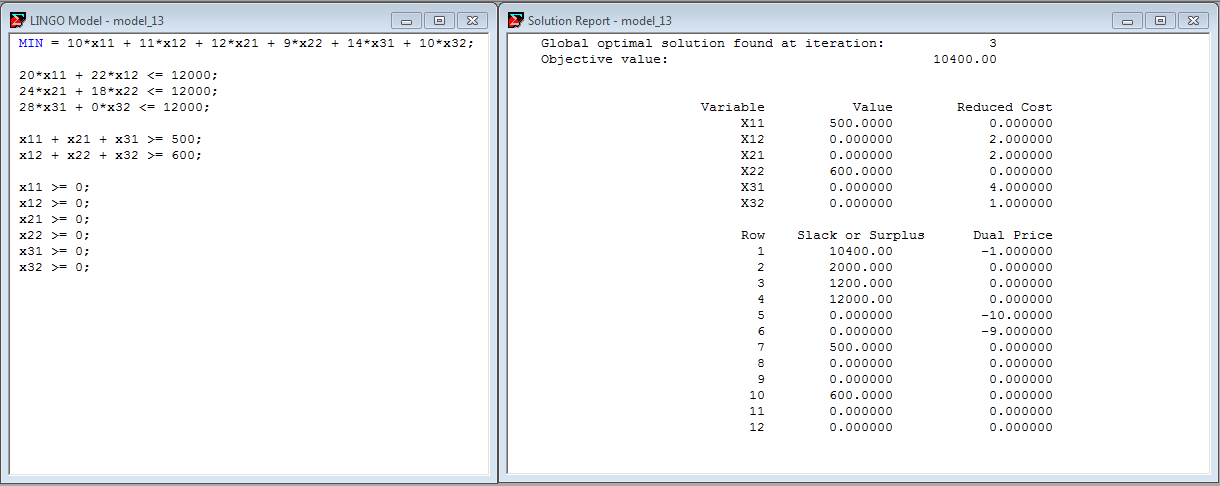
\includegraphics[width=300px]{slides/ex13/screenshot.png}
    \caption{Example 13 model and solution in Lingo Software.}
\end{figure}
\end{frame}

\begin{frame}{Example 13 - Final solution}
\footnotesize
\colorb{Global optimal solution found at iteration:}  0\\
\colorb{Objective value:}  760.0000\\

\begin{columns}[t]
\begin{column}{0.3\textwidth}
\colorb{Variable}\\
HO\\
HOP\\
FP\\
F\\
O\\
-----------\\
\colorb{Row}\\
1\\
2\\
3\\
4\\
5\\
6\\
7\\
8\\
9\\
10\\

\end{column}
\begin{column}{0.3\textwidth}
\colorb{Value}\\
10.00000\\
0.000000\\
8.000000\\
2.000000\\
20.00000\\
-----------\\
\colorb{Slack or Surplus}\\
760.0000\\
0.000000\\
0.000000\\
0.000000\\
0.000000\\
20.00000\\
10.00000\\
0.000000\\
8.000000\\
2.000000\\
\end{column}  

\begin{column}{0.3\textwidth}
\colorb{Reduced Cost}\\
0.000000\\
2.500000\\
0.000000\\
0.000000\\
0.000000\\
-----------\\
\colorb{Dual Price}\\
1.000000\\
10.00000\\
60.00000\\
40.00000\\
1.166667\\
0.000000\\
0.000000\\
0.000000\\
0.000000\\
0.000000\\
\end{column}
\end{columns}  
\end{frame}

\begin{frame}{Example 13 - Final analisis}
\end{frame}



%\begin{frame}{}
\begin{center}
{\Huge Example 14}
\end{center}
\end{frame}

\begin{frame}{Example 14 - Problem}
\end{frame}

\begin{frame}{Example 14 - Analisis}
\end{frame}

\begin{frame}{Example 14 - Variables}
\end{frame}

\begin{frame}{Example 14 - Function}

Minimize the cost of Steelco of manufacturing the two types of steel:
\begin{align*}
    Z =& 10\colorij{X}{1}{1} + 11\colorij{X}{1}{2} + 12\colorij{X}{2}{1} +
          9\colorij{X}{2}{2} + 14\colorij{X}{3}{1} + 10\colorij{X}{3}{2}
\end{align*}

\end{frame}

\begin{frame}{Example 14 - Restrictions}
\end{frame}

\begin{frame}{Example 14 - Model}
\end{frame}

\begin{frame}{Example 14 - Solution(1)}
\begin{figure}
    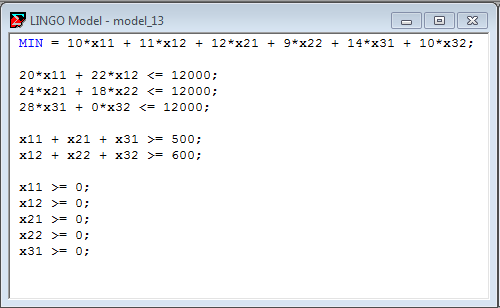
\includegraphics[width=300px]{slides/ex14/screenshot_a.png}
    \caption{Example 14 model and solution in Lingo Software.}
\end{figure}
\end{frame}

\begin{frame}{Example 14 - Solution(2)}
\begin{figure}
    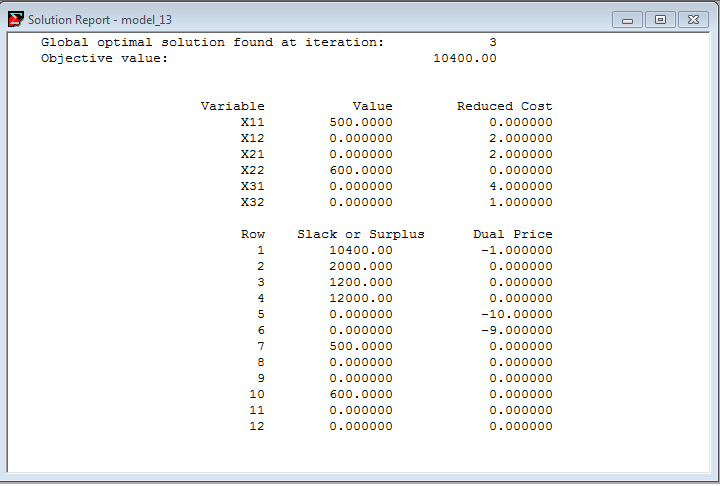
\includegraphics[width=300px]{slides/ex14/screenshot_b.png}
    \caption{Example 14 model and solution in Lingo Software.}
\end{figure}
\end{frame}


\begin{frame}{Example 14 - Final solution}
\end{frame}

\begin{frame}{Example 14 - Final analisis}
\end{frame}



%\begin{frame}{}
\begin{center}
{\Huge Example 15}
\end{center}
\end{frame}

\begin{frame}{Example 15 - Problem (1)}
Kiriakis Electronics produces three products. Each product must be processed on
each of three types of machines. When a machine is in use, it must be manned
by a worker. The time (in hours) required to process each product on each
machine and the profit associated with each product are shown in following
table.

\begin{center}
\begin{tabular}{lrrr}
\hline
  \cellcolor{gray90}\textbf{Machine}
& \cellcolor{gray90}\textbf{Product 1}
& \cellcolor{gray90}\textbf{Product 2}
& \cellcolor{gray90}\textbf{Product 3} \\
\hline
Machine 1 & 2 & 3 & 4 \\
Machine 2 & 3 & 5 & 6 \\
Machine 3 & 4 & 7 & 9 \\
\hline
Profit & \$6 & \$8 & \$10 \\
\hline
\end{tabular}
\end{center}

\end{frame}

\begin{frame}{Example 15 - Problem (2)}
At present, five type 1 machines, three type 2 machines, and four type 3
machines are available. The company has ten workers available and must determine
how many workers to assign to each machine. The plant is open 40 hours per week,
and each worker works 35 hours per week. Formulate an LP that will enable
Kiriakis to assign workers to machines in a way that maximizes weekly profits. \\
\vspace{3mm}
{\small \textbf{Note}:
a worker need not spend the entire work week manning a single machine.
}
\end{frame}


\begin{frame}{Example 15 - Analisis}

Kiriakis wants to maximize weekly profits and each type of product
yields different profits.Product 1 yields \$6, product 2 yields \$8 and
product 3 yields \$10 . So it's about maximize the sum of
Product Profit * Product\_i, where i refers to type of product.
\end{frame}

\begin{frame}{Example 15 - Variables}
\end{frame}

\begin{frame}{Example 15 - Function}

Enable Kiriakis Electronics to assign workers to machines
in a way that maximizes weekly profits:
\begin{align*}
    Z &= 6\colora{X_1} + 8\colorb{X_2} + 10\colorc{X_3}
\end{align*}


\end{frame}

\begin{frame}{Example 15 - Restrictions (1)}

The first restriction is given by the hours that are required for each product
in the machine 1. Knowing that there are 5 machines of this type available and
that the factory is open 40 hours, therefore with the hours given in the board
of the machine 1 we have that 2
$2\colora{X_1} +  3\colorb{X_2} +  4\colorc{X_3} \le 200$. Similarly a
restriction of the same nature is obtained for the other remaining two machines:
for machine 2 we have $3\colora{X_1} +  5\colorb{X_2} +  6\colorc{X_3} \le 120$
for there are 3 machines available. For the machine 3 we have
$4\colora{X_1} +  7\colorb{X_2} +  9\colorc{X_3} \le 160$
for there are 4 machines available.

\end{frame}


\begin{frame}{Example 15 - Restrictions (2)}

There is also the restriction of each worker working a total of 35 hours per
week for a total of 10 workers and when each product is in a machine it must be
handled by a worker, because of this all the hours required by product are
added, so for product 1 9 hours are required; for product 2, 15 hours and for
product 3 19 hours from what we obtain:
$9\colora{X_1} + 15\colorb{X_2} + 19\colorc{X_3} \le 350$. Finally there is the
trivial restriction that no negative products can exits.

\end{frame}

\begin{frame}{Example 15 - Model}
\end{frame}

\begin{frame}{Example 15 - Solution}
\end{frame}

\begin{frame}{Example 15 - Final solution}
\footnotesize
\colorb{Global optimal solution found at iteration:} 1 \\
\colorb{Objective value:}  233.3333\\

\begin{columns}[t]
\begin{column}{0.3\textwidth}
\colorb{Variable}\\
X1\\
X2\\
X3\\
-----------\\
\colorb{Row}\\
1\\
2\\
3\\
4\\
5\\
6\\
7\\
8\\

\end{column}
\begin{column}{0.3\textwidth}
\colorb{Value}\\
38.88889\\
0.000000\\
0.000000\\

-----------\\
\colorb{Slack or Surplus}\\
233.3333\\
122.2222\\
3.333333\\
4.444444\\
0.000000\\
38.88889\\
0.000000\\
0.000000\\

\end{column}  

\begin{column}{0.3\textwidth}
\colorb{Reduced Cost}\\
0.000000\\
2.000000\\
2.666667\\

-----------\\
\colorb{Dual Price}\\
1.000000\\
0.000000\\
0.000000\\
0.000000\\
0.6666667\\
0.000000\\
0.000000\\
0.000000\\
\end{column}
\end{columns}  
\end{frame}

\begin{frame}{Example 15 - Final analisis}
%Kiriakis Electronics, 3 products,3 machines
LINGO give the optimal solution that says that Kiriakis must produce
38.88889 products type 1 and 0 products type 2 and type 3, otherwise
the profits will decrease by \$2 per product 2 or \$2.67 per product 3.
The optimal profit ok Kiriakis is of \$233.3333.
\end{frame}



%\begin{frame}{}
\begin{center}
{\Huge Example 16}
\end{center}
\end{frame}

\begin{frame}{Example 16 - Problem (1)}
Oliver Winery produces four award-winning wines in Bloomington, Indiana. The
profit contribution, labor hours, and tank usage (in hours) per gallon for each
type of wine are given in the following table.

\begin{center}
\begin{tabular}{lrrr}
\hline
  \cellcolor{gray90}\textbf{Wine}
& \cellcolor{gray90}\textbf{Profit}
& \cellcolor{gray90}\textbf{Labor}
& \cellcolor{gray90}\textbf{Tank} \\
\hline
Wine 1 &  \$6 & .2 hr &  .5 hr \\
Wine 2 & \$12 & .3 hr &  .5 hr \\
Wine 3 & \$20 & .3 hr & 1   hr \\
Wine 4 & \$30 & .5 hr & 1.5 hr \\
\hline
\end{tabular}
\end{center}

\end{frame}

\begin{frame}{Example 16 - Problem (2)}
By law at most 100000 gallons of wine can be produced each year. A maximum of
12000 labor hours and 32000 tank hours are available annually. Each gallon of
wine 1 spends an average of (1/2) year in inventory; wine 2, an average of 1
year; wine 3, an average of 2 years; wine 4, an average of 3.333 years. The
winery's warehouse can handle an average inventory level of 50000 gallons.
Determine how much of each type of wine should be produced annually to maximize
OliverWinery's profit.
\end{frame}

\begin{frame}{Example 16 - Analisis}
\end{frame}

\begin{frame}{Example 16 - Variables}
\end{frame}

\begin{frame}{Example 16 - Function}

Maximize Oliver Winery's profit by determining how much of each
type of wine should be produced anually:
\begin{align*}
    Z &= 6\colora{W_1} + 12\colorb{W_2} + 20\colorc{W_3} + 30\colord{W_4}
\end{align*}

\end{frame}

\begin{frame}{Example 16 - Restrictions}

%FIXME: Explain
\begin{align*}
       \colora{W_1} +    \colorb{W_2} +    \colorc{W_3} +    \colord{W_4} &\le 100000 \\
    0.2\colora{W_1} + 0.3\colorb{W_2} + 0.3\colorc{W_3} + 0.5\colord{W_4} &\le 12000 \\
    0.5\colora{W_1} + 0.5\colorb{W_2} +    \colorc{W_3} + 1.5\colord{W_4} &\le 32000 \\
    \frac{1}{3}\colora{W_1} + \colorb{W_2} + 2\colorc{W_3} + \frac{1}{3}\colord{W_4} &\le 50000 \\
    \colora{W_1}, \colorb{W_2}, \colorc{W_3}, \colord{W_4} &\ge 0
\end{align*}

\end{frame}

\begin{frame}{Example 16 - Model}

Maximize:
\begin{align*}
    Z &= 6\colora{W_1} + 12\colorb{W_2} + 20\colorc{W_3} + 30\colord{W_4}
\end{align*}

Subject to:
\begin{align*}
       \colora{W_1} +    \colorb{W_2} +    \colorc{W_3} +    \colord{W_4} &\le 100000 \\
    0.2\colora{W_1} + 0.3\colorb{W_2} + 0.3\colorc{W_3} + 0.5\colord{W_4} &\le 12000 \\
    0.5\colora{W_1} + 0.5\colorb{W_2} +    \colorc{W_3} + 1.5\colord{W_4} &\le 32000 \\
    \frac{1}{3}\colora{W_1} + \colorb{W_2} + 2\colorc{W_3} + \frac{1}{3}\colord{W_4} &\le 50000 \\
    \colora{W_1}, \colorb{W_2}, \colorc{W_3}, \colord{W_4} &\ge 0
\end{align*}

\end{frame}

\begin{frame}{Example 16 - Solution}
\end{frame}

\begin{frame}{Example 16 - Final solution}
\footnotesize
\colorb{Global optimal solution found at iteration:}  4\\
\colorb{Objective value:}  574000.0\\

\begin{columns}[t]
\begin{column}{0.3\textwidth}

\colorb{Variable}\\
W1\\
W2\\
W3\\
W4\\
-----------\\
\colorb{Row}\\
1\\
2\\
3\\
4\\
5\\

\end{column}
\begin{column}{0.3\textwidth}

\colorb{Value}\\
21000.00\\
9000.000\\
17000.00\\
0.000000\\


-----------\\
\colorb{Slack or Surplus}\\
574000.0\\
53000.00\\
0.000000\\
0.000000\\
0.000000\\

\end{column}

\begin{column}{0.3\textwidth}

\colorb{Reduced Cost}\\
0.000000\\
0.000000\\
0.000000\\
2.997667\\

-----------\\
\colorb{Dual Price}\\
1.000000\\
0.000000\\
13.33333\\
2.000000\\
7.000000\\
\end{column}
\end{columns}
\end{frame}

\begin{frame}{Example 16 - Final analisis}
\end{frame}



%\begin{frame}{}
\begin{center}
{\Huge Example 17}
\end{center}
\end{frame}

\begin{frame}{Example 17 - Problem}
\end{frame}

\begin{frame}{Example 17 - Analisis}
\end{frame}

\begin{frame}{Example 17 - Variables}
\begin{center}
\Huge{
$\colora{X}_{\colorb{i}}$ \\
}
\end{center}
\LARGE{
$\colora{C} \longrightarrow$
    tellers grouped by shifts \\
$\colorb{i} \longrightarrow$
    shifts
}
\end{frame}

\begin{frame}{Example 17 - Function}
\end{frame}

\begin{frame}{Example 17 - Restrictions}
\end{frame}

\begin{frame}{Example 17 - Model}

Minimize:
\begin{align*}
    Z &= 64(\colorsub{X}{1} + \colorsub{X}{2}) +
         15(\colorsub{X}{3} + \colorsub{X}{4} + \colorsub{X}{5} +
            \colorsub{X}{6} + \colorsub{X}{7} + \colorsub{X}{8})
\end{align*}

Subject to:
\begin{align*}
    \colorsub{X}{3} + \colorsub{X}{4} + \colorsub{X}{5} +
    \colorsub{X}{6} + \colorsub{X}{7} + \colorsub{X}{8} &\le 5 \\
    \colorsub{X}{1} + \colorsub{X}{2} + \colorsub{X}{3} &= 4 \\
    \colorsub{X}{1} + \colorsub{X}{2} + \colorsub{X}{3} + \colorsub{X}{4} &= 3 \\
    \colorsub{X}{1} + \colorsub{X}{2} + \colorsub{X}{3} + \colorsub{X}{4} + \colorsub{X}{5} &= 4 \\
    \colorsub{X}{2} + \colorsub{X}{4} + \colorsub{X}{5} + \colorsub{X}{6} &= 6 \\
    \colorsub{X}{1} + \colorsub{X}{5} + \colorsub{X}{6} + \colorsub{X}{7} &= 5 \\
    \colorsub{X}{1} + \colorsub{X}{2} + \colorsub{X}{6} + \colorsub{X}{7} + \colorsub{X}{8} &= 6 \\
    \colorsub{X}{1} + \colorsub{X}{2} + \colorsub{X}{7} + \colorsub{X}{8} &= 8 \\
    \colorsub{X}{1} + \colorsub{X}{2} + \colorsub{X}{6} + \colorsub{X}{8} &= 8 \\
    \colorsub{X}{i} &\ge 0
\end{align*}

\end{frame}

\begin{frame}{Example 17 - Solution}
\end{frame}

\begin{frame}{Example 17 - Final solution (1)}
\footnotesize
\colorb{Global optimal solution found at iteration:} \\
\colorb{Objective value:}  \\

\begin{columns}[t]
\begin{column}{0.3\textwidth}
\colorb{Variable}\\
X1\\
X2\\
X3\\
X4\\
X5\\
X6\\
X7\\
X8\\
\end{column}
\begin{column}{0.3\textwidth}
\colorb{Value}\\
0.000000\\
4.000000\\
0.000000\\
-1.000000\\
1.000000\\
1.000000\\
3.000000\\
1.000000\\
\end{column}

\begin{column}{0.3\textwidth}
\colorb{Reduced Cost}\\
0.000000\\
0.000000\\
0.3200000E+12\\
0.6400000E+11\\
0.000000\\
0.000000\\
0.000000\\
0.000000\\
\end{column}
\end{columns}
\end{frame}


\begin{frame}{Example 17 - Final solution (2)}
\footnotesize

\begin{columns}[t]
\begin{column}{0.3\textwidth}
\colorb{Row}\\
1\\
2\\
3\\
4\\
5\\
6\\
7\\
8\\
9\\
\end{column}
\begin{column}{0.3\textwidth}
\colorb{Slack or Surplus}\\
0.000000\\
0.000000\\
0.000000\\
0.000000\\
0.000000\\
-1.000000\\
0.000000\\
-3.000000\\
0.000000\\
\end{column}

\begin{column}{0.3\textwidth}
\colorb{Dual Price}\\
-1.000000\\
0.1280000E+12\\
0.1280000E+12\\
0.6400000E+11\\
0.000000\\
-0.6400000E+11\\
-0.6400000E+11\\
0.6400000E+11\\
-0.1280000E+12\\
\end{column}
\end{columns}
\end{frame}

\begin{frame}{Example 17 - Final solution (3)}
\footnotesize
\begin{columns}[t]
\begin{column}{0.3\textwidth}
\colorb{Row}\\
10\\
11\\
12\\
13\\
14\\
15\\
16\\
17\\
18\\

\end{column}
\begin{column}{0.3\textwidth}
\colorb{Slack or Surplus}\\
-2.000000\\
0.000000\\
4.000000\\
0.000000\\
-1.000000\\
1.000000\\
1.000000\\
3.000000\\
1.000000\\

\end{column}

\begin{column}{0.3\textwidth}
\colorb{Dual Price}\\
-0.6400000E+11\\
0.000000\\
0.000000\\
0.000000\\
-0.6400000E+11\\
0.000000\\
0.000000\\
0.000000\\
0.000000\\

\end{column}
\end{columns}
\end{frame}

\begin{frame}{Example 17 - Final analisis}
\end{frame}



%\begin{frame}{}
\begin{center}
{\Huge Example 18}
\end{center}
\end{frame}

\begin{frame}{Example 18 - Problem}
\end{frame}

\begin{frame}{Example 18 - Analisis}
\end{frame}

\begin{frame}{Example 18 - Variables}
\end{frame}

\begin{frame}{Example 18 - Function}
\end{frame}

\begin{frame}{Example 18 - Restrictions}
\end{frame}

\begin{frame}{Example 18 - Model}

Minimize:
\begin{align*}
    Z =& 5\colorsub{M}{1} + 6\colorsub{M}{2} + 8\colorsub{M}{3} + 10\colorsub{M}{4} + \\
       & 20\colorsub{D}{1} + 20\colorsub{D}{2} + 20\colorsub{D}{3} + 20\colorsub{D}{4} + \\
       & 15\colorsub{DA}{1} + 15\colorsub{DA}{2} + 15\colorsub{DA}{3} + 15\colorsub{DA}{4}
\end{align*}

Subject to:
\vspace{-1cm}
\begin{multicols}{2}
\tiny{
\begin{align*}
    \colorsub{D}{1} + \colorsub{DA}{1} &\le \colorsub{M}{1} \\
    \colorsub{D}{2} + \colorsub{DA}{2} &\le \colorsub{M}{2} \\
    \colorsub{D}{3} + \colorsub{DA}{3} &\le \colorsub{M}{3} \\
    \colorsub{D}{4} + \colorsub{DA}{4} &\le \colorsub{M}{4} \\
    %
    (0.15 * 0.90)\colorsub{D}{1} + (0.15 * 0.80)\colorsub{DA}{1} &= \colorsub{P}{1} \\
    (0.20 * 0.90)\colorsub{D}{2} + (0.15 * 0.80)\colorsub{DA}{2} &= \colorsub{P}{2} \\
    (0.30 * 0.90)\colorsub{D}{3} + (0.15 * 0.80)\colorsub{DA}{3} &= \colorsub{P}{3} \\
    (0.40 * 0.90)\colorsub{D}{4} + (0.15 * 0.80)\colorsub{DA}{4} &= \colorsub{P}{4} \\
    %
    \colorsub{M}{i}, \colorsub{P}{i}, \colorsub{D}{i}, \colorsub{DA}{i} &\ge 0 \\
    \colorij{PG}{i}{j} &\ge 0
\end{align*}
}

\vfill
\columnbreak

\tiny{
\begin{align*}
    \colorsub{D}{1} + \colorsub{D}{2} +
    \colorsub{D}{3} + \colorsub{D}{4} &\le 3000 \\
    %
    \colorsub{DA}{1} + \colorsub{DA}{2} +
    \colorsub{DA}{3} + \colorsub{DA}{4} &\le 3000 \\
    %
    \colorij{PG}{2}{2} + \colorij{PG}{1}{3} &\le \colorsub{P}{1} \\
    \colorij{PG}{3}{2} + \colorij{PG}{2}{3} &\le \colorsub{P}{2} \\
    \colorij{PG}{3}{2} + \colorij{PG}{3}{3} &\le \colorsub{P}{3} \\
    \colorij{PG}{4}{2} + \colorij{PG}{4}{3} &\le \colorsub{P}{4} \\
    %
    \colorij{PG}{3}{1} + \colorij{PG}{4}{1} &\ge 500 \\
    \colorij{PG}{1}{2} + \colorij{PG}{2}{2} + \colorij{PG}{4}{2} &\ge 500 \\
    \colorij{PG}{1}{3} + \colorij{PG}{2}{3} + \colorij{PG}{3}{3} &\ge 500
    %
\end{align*}
}
\end{multicols}

\end{frame}

\begin{frame}{Example 18 - Solution (1)}
\begin{figure}
    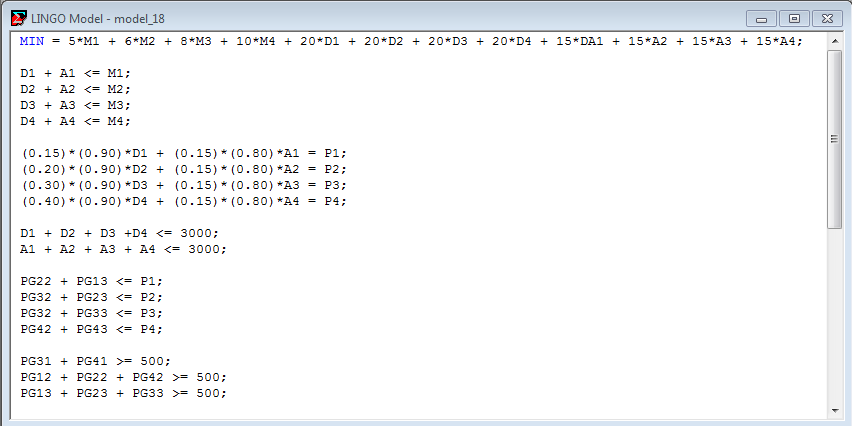
\includegraphics[width=300px]{slides/ex18/screenshot_a.png}
    \caption{Example 18 model and solution in Lingo Software.}
\end{figure}
\end{frame}

\begin{frame}{Example 18 - Solution (2)}
\begin{figure}
    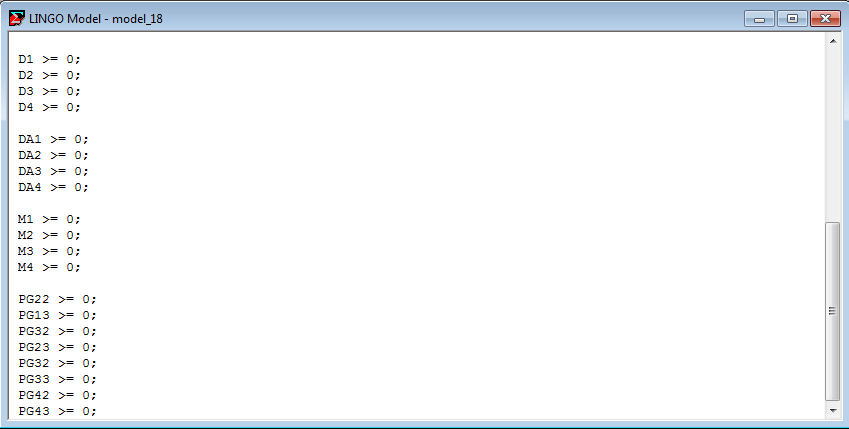
\includegraphics[width=300px]{slides/ex18/screenshot_b.png}
    \caption{Example 18 model and solution in Lingo Software.}
\end{figure}
\end{frame}

\begin{frame}{Example 18 - Solution (3)}
\begin{figure}
    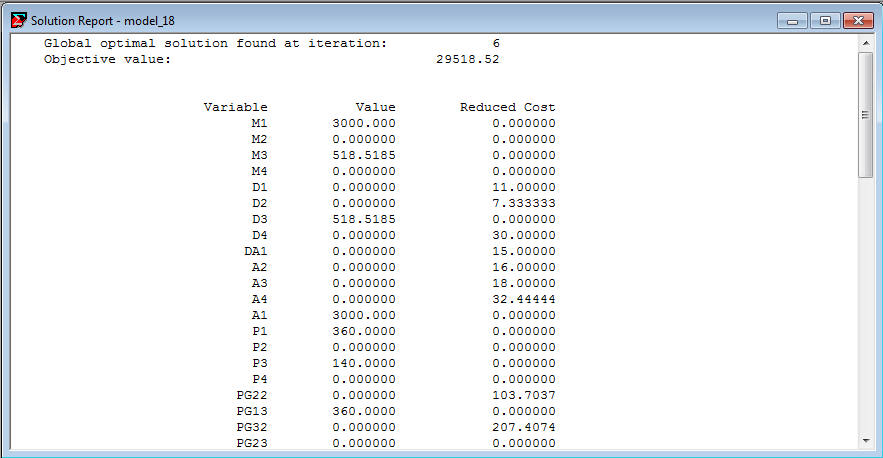
\includegraphics[width=300px]{slides/ex18/screenshot_c.png}
    \caption{Example 18 model and solution in Lingo Software.}
\end{figure}
\end{frame}

\begin{frame}{Example 18 - Solution (4)}
\begin{figure}
    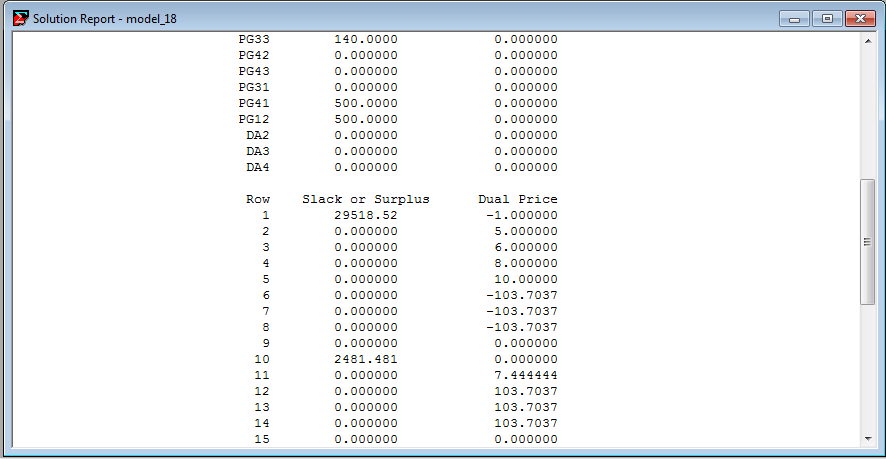
\includegraphics[width=300px]{slides/ex18/screenshot_d.png}
    \caption{Example 18 model and solution in Lingo Software.}
\end{figure}
\end{frame}

\begin{frame}{Example 18 - Solution (5)}
\begin{figure}
    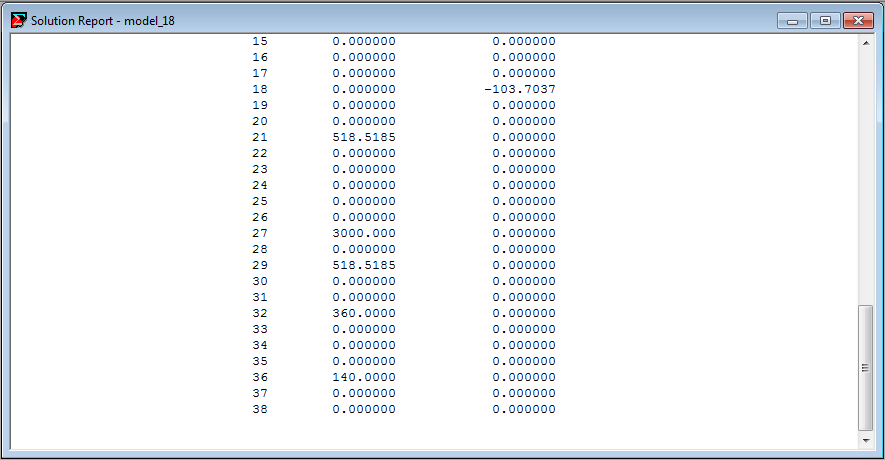
\includegraphics[width=300px]{slides/ex18/screenshot_e.png}
    \caption{Example 18 model and solution in Lingo Software.}
\end{figure}
\end{frame}



\begin{frame}{Example 18 - Final solution}

\colorb{Global optimal solution found at iteration:} \\
\colorb{Objective value:}  \\

\begin{columns}[t]
\begin{column}{0.3\textwidth}
\colorb{Variable}\\

-----------\\
\colorb{Row}\\


\end{column}
\begin{column}{0.3\textwidth}
\colorb{Value}\\


-----------\\
\colorb{Slack or Surplus}\\


\end{column}  

\begin{column}{0.3\textwidth}
\colorb{Reduced Cost}\\


-----------\\
\colorb{Dual Price}\\

\end{column}
\end{columns}
\end{frame}

\begin{frame}{Example 18 - Final analisis}
According to LINGO solution, the recycling plant must purchase 3000 raw material 1, 0 raw material 2
and 516.518 raw material 3, the same amount is processed by de-inking. 3000 tons of materials will be processed
using asphalt dispersion. It will be produced 360 tons of pulp 1 , 140 of pulp 3 and finally, there are
360 tons of pulp 1 for paper grade 3, 140 tons of pulp 3 for paper grade 3 and 500 tons of pulp 4
for paper grade 1. So the cost of meeting these demands is of \$29518.52.
\end{frame}



%\begin{frame}{}
\begin{center}
{\Huge Example 19}
\end{center}
\end{frame}

\begin{frame}{Example 19 - Problem}
\end{frame}

\begin{frame}{Example 19 - Analisis}
\end{frame}

\begin{frame}{Example 19 - Variables}
\end{frame}

\begin{frame}{Example 19 - Function}
\end{frame}

\begin{frame}{Example 19 - Restrictions}
\end{frame}

\begin{frame}{Example 19 - Model}
\end{frame}

\begin{frame}{Example 19 - Solution}
\begin{figure}
    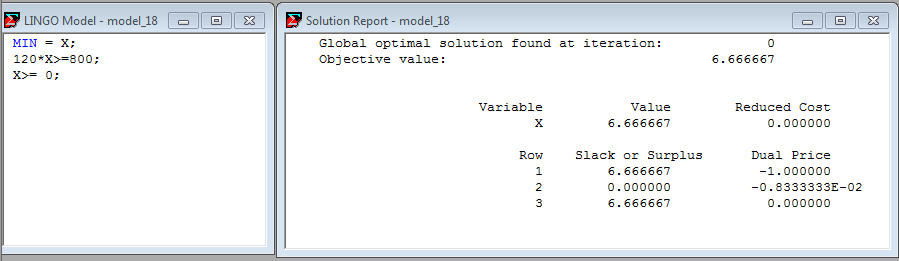
\includegraphics[width=300px]{slides/ex19/screenshot.png}
    \caption{Example 19 model and solution in Lingo Software.}
\end{figure}
\end{frame}

\begin{frame}{Example 19 - Final solution}

\colorb{Global optimal solution found at iteration:}  0\\
\colorb{Objective value:}  6.666667\\

\begin{columns}[t]
\begin{column}{0.3\textwidth}
\colorb{Variable}\\
X\\
-----------\\
\colorb{Row}\\
1\\
2\\
3\\

\end{column}
\begin{column}{0.3\textwidth}
\colorb{Value}\\
6.666667\\

-----------\\
\colorb{Slack or Surplus}\\
6.666667\\
0.000000\\
6.666667\\

\end{column}  

\begin{column}{0.3\textwidth}
\colorb{Reduced Cost}\\
0.000000\\

-----------\\
\colorb{Dual Price}\\
-1.000000\\
-0.8333333E\\
0.000000\\
\end{column}
\end{columns}
\end{frame}

\begin{frame}{Example 19 - Final analisis}
The solution given by LINGO says that Llanview needs around 6.666667 judges.
\end{frame}



%\begin{frame}{}
\begin{center}
{\Huge Example 20}
\end{center}
\end{frame}

\begin{frame}{Example 20 - Problem (1)}
Olé Oil produces three products: heating oil, gasoline, and jet fuel. The
average octane levels must be at least 4.5 for heating oil, 8.5 for gas and
7.0 for jet fuel. To produce these products Olé purchases two types of oil:
crude 1 (at \$12 per barrel) and crude 2 (at \$10 per barrel). Each day, at
most 10000 barrels of each type of oil can be purchased.
\end{frame}

\begin{frame}{Example 20 - Problem (2)}
Before crude can be used to produce products for sale it must be distilled.
Each day, at most 15000 barrels of oil can be distilled. It cost 10\$ to distill
a barrel of oil. The result of distillation is as follows: (1) Each barrel of
crude 1 yields 0.6 barrel of naphtha, 0.3 barrel of distilled 1, and 0.1 barrel
of distilled 2. (2) Each barrel of crude 2 yields 0.4 barrel of naphtha, 0.2
barrel of distilled 1, and 0.4 barrel of distilled 2. Distilled naphtha can be
used only to produce gasoline or jet fuel. Distilled oil can be used to produce
heating oil or it can be sent through the catalytic cracker (at a cost of 15\$
per barrel). Each day, at most 5000 barrels of distilled oil can be sent
through the cracker.
\end{frame}

\begin{frame}{Example 20 - Problem (3)}
Each barrel of distilled 1 sent through the cracker yields
0.8 barrel of cracked 1and 0.2 barrel of cracked 2. Each barrel of distilled 2
sent through the cracker yields 0.7 barrel of cracked 1 and 0.3 barrel of
cracked 2. Cracked oil can be used to produce gasoline and jet fuel but no to
produce heating oil.\\
\vspace{3mm}
The octane level of each type of oil is as follows: naphtha, 8; distilled 1, 4;
distilled 2, 5; cracked 1, 9; cracked 2, 6. \\
\vspace{3mm}
All heating oil produced can be sold at \$14 per barrel; all gasoline produced,
\$18 per barrel; and all jet fuel produced \$16 per barrel. Marketing
considerations dictate that at least 3000 barrels of each product must be
produced daily. Formulate an LP to maximize Olé’s daily profit.
\end{frame}

\begin{frame}{Example 20 - Analisis}
\end{frame}

\begin{frame}{Example 20 - Variables}
\small{
$C1  \longrightarrow$ amount of crude 1 barrels bought for distillation \\
$C2  \longrightarrow$ amount of crude 2 barrels bought for distillation \\
$NG  \longrightarrow$ amount of naphtha barrels produced for gasoline \\
$NJF \longrightarrow$ amount of naphtha barrels produced for jet fuel \\
$X_{d1ho} \longrightarrow$ amount of distillated 1 oil barrels produced for heating oil \\
$X_{d1c} \longrightarrow$ amount of distillated 1 oil barrels produced for cracker \\
$X_{d2ho} \longrightarrow$ amount of distillated 2 oil barrels produced for heating oil \\
$X_{d2c} \longrightarrow$ amount of distillated 2 oil barrels produced for cracker \\
$X_{co1g} \longrightarrow$ amount of crack oil 1 barrels produced for gasoline \\
$X_{co1ho} \longrightarrow$ amount of crack oil 1 barrels produced for heating oil \\
$X_{co2g} \longrightarrow$ amount of crack oil 2 barrels produced for gasoline \\
$X_{co2ho} \longrightarrow$ amount of crack oil 2 barrels produced for heating oil
}
\end{frame}

\begin{frame}{Example 20 - Function}
\end{frame}

\begin{frame}{Example 20 - Restrictions}

%FIXME: Explain.
\begin{multicols}{2}
\tiny{
\begin{align*}
    C1 &\le 10000 \\
    C2 &\le 10000 \\
    C1 + C2 &\le 15000 \\
    %
    NG + NJF - 0.6C1 - 0.4C2 &= 0 \\
    %
    X_{d1c} + X_{d1ho} - 0.3C1 - 0.2C2 &= 0 \\
    X_{d2c} + X_{d2ho} - 0.1C1 - 0.4C2 &= 0 \\
    X_{d1c} + X_{d2c} &\le 5000 \\
    X_{k} &\ge 0
\end{align*}
}

\vfill
\columnbreak

\tiny{
\begin{align*}
    X_{co1g} + X_{co1ho} - 0.8X_{d1c} - 0.7X_{d2c} &= 0 \\
    X_{co1g} + X_{co1ho} - 0.3X_{d1c} - 0.2X_{d2c} &= 0 \\
    %
    9X_{co1g} + 6X_{co2g} + 8NG &\ge 8.5 \\
    4X_{d1ho} + 5X_{d2ho} &\ge 4.5 \\
    9X_{co1j} + 6X_{co2j} + 8NJF &\ge 7.0 \\
    X_{co1g} + X_{co2g} + NG &\ge 3000 \\
    X_{d1ho} + X_{d2ho} &\ge 3000 \\
    X_{co1j} + X_{co2j} + NJF &\ge 3000
\end{align*}
}
\end{multicols}

\end{frame}

\begin{frame}{Example 20 - Model}

Minimize:
\begin{align*}
    Z =& 17.75X_{co1g} + 15.75X_{co1j} + \\
       & 17.75X_{co2g} + 15.75X_{co2j} + \\
       & 17.9NG + 15.9NJF + \\
       & 13.9X_{d1ho} + 13.9X_{d2ho} - \\
       & 12C1 - 10C2
\end{align*}

Subject to:
\vspace{-1cm}
\begin{multicols}{2}
\tiny{
\begin{align*}
    C1 &\le 10000 \\
    C2 &\le 10000 \\
    C1 + C2 &\le 15000 \\
    %
    NG + NJF - 0.6C1 - 0.4C2 &= 0 \\
    %
    X_{d1c} + X_{d1ho} - 0.3C1 - 0.2C2 &= 0 \\
    X_{d2c} + X_{d2ho} - 0.1C1 - 0.4C2 &= 0 \\
    X_{d1c} + X_{d2c} &\le 5000 \\
    X_{k} &\ge 0
\end{align*}
}

\vfill
\columnbreak

\tiny{
\begin{align*}
    X_{co1g} + X_{co1ho} - 0.8X_{d1c} - 0.7X_{d2c} &= 0 \\
    X_{co1g} + X_{co1ho} - 0.3X_{d1c} - 0.2X_{d2c} &= 0 \\
    %
    9X_{co1g} + 6X_{co2g} + 8NG &\ge 8.5 \\
    4X_{d1ho} + 5X_{d2ho} &\ge 4.5 \\
    9X_{co1j} + 6X_{co2j} + 8NJF &\ge 7.0 \\
    X_{co1g} + X_{co2g} + NG &\ge 3000 \\
    X_{d1ho} + X_{d2ho} &\ge 3000 \\
    X_{co1j} + X_{co2j} + NJF &\ge 3000
\end{align*}
}
\end{multicols}

\end{frame}

\begin{frame}{Example 20 - Solution}
\end{frame}

\begin{frame}{Example 20 - Final solution}
\end{frame}

\begin{frame}{Example 20 - Final analisis}
\end{frame}




\end{document}
